%\documentclass[10pt,a4paper]{article}
%\usepackage[latin1]{inputenc}
%\usepackage{amsmath}
%\usepackage{amsfonts}
%\usepackage{amssymb}
%\usepackage{graphicx}

% igs2ejournalguide.tex
% v4.00 3-sept-2015

\NeedsTeXFormat{LaTeX2e}

% check that the math fits the two-column format:
% \documentclass[twocolumn]{igs}

% but use this version when submitting your article:
\documentclass[review,oneside]{igs}

% other options are available
%   authors printing on US letter size are advised 
%   to use the slightly shorter [letterpaper] option
% SINGLE COLUMN
%   \documentclass{igs}              
% SINGLE COLUMN, FEWER LINES/PAGE
%   \documentclass[letterpaper]{igs} 
% DOUBLE COLUMN, FEWER LINES/PAGE
%   \documentclass[twocolumn,letterpaper]{igs} 

\usepackage{igsnatbib}
\usepackage{appendix}

% check if we are compiling under latex or pdflatex
\ifx\pdftexversion\undefined
\usepackage[dvips]{graphicx}
\else
\usepackage[pdftex]{graphicx}
\usepackage{epstopdf}
\epstopdfsetup{suffix=}
\fi

% the default is for unnumbered section heads
% if you really must have numbered sections, remove
% the % from the beginning of the following command
% and insert the level of sections you wish to be
% numbered (up to 4):

% \setcounter{secnumdepth}{2}

\begin{document}
\title{Diagnosising the sensitivity of grounding line flux to changes in sub-ice shelf melting}

\author[Zhang and others]{Tong Zhang, Stephen Price, Matthew Hoffman, Xylar Asay-Davis}
\affiliation{%
  Fluid Dynamics and Solid Mechanics Group, Los Alamos National Laboratory, New Mexico, United States, 87545\\
  Correspondence: Tong Zhang 
  $<$tzhang@lanl.gov$>$}
 
\abstract{Motivated by previous work using ice flow models to quantify ice shelf buttressing and its impacts on the flux of ice across the grounding line \citep[e.g.,][]{furst2016,reese2018}, we seek an improved physical understanding for how ice dynamics link small ice thickness perturbations, via changes in sub-ice shelf melting, to changes in ice shelf buttressing and ice flux across the grounding line. More specifically, we seek to define one or more ``metrics'' that are 1) readily calculated from standard ice sheet model outputs and 2) informative for diagnosing the sensitivity of grounding line flux to changes in ice thickness at specific locations on an ice shelf. By studying the ice dynamics for both idealized (MISMIP+) and realistic (Larsen C) ice shelves, we find that the first principle stress is the best overall metric for linking local changes in ice shelf thickness and dynamics with changes in the integrated grounding line flux. Unfortunately, this metric only shows a robust relationship with the integrated grounding line flux for regions near the center of an ice shelf; for points too near the grounding line or the calving front, no clear relationship exists between any of the readily calculable metrics explored here and changes in grounding line flux. This motivates our exploration of an adjoint-based method for defining grounding line flux sensitivity to local changes in ice shelf geometry. Using the same idealized and realistic test cases, we demonstrate that this method is equivalent to the sensitivity analysis of \citep{reese2018} but requires only a single model adjoint solve. We conclude that the adjoint-based method can provide a means of analyzing grounding line flux sensitivity to changes in sub-ice shelf melting at model run time.}

\maketitle


\section{Introduction}

Marine ice sheets like West Antarctica (and to a lesser extent, portions of East Antarctica) are grounded below sea level and their bedrock would remain so even after full isostatic rebound \citep{barletta2018}. This and the fact that ice sheets generally thicken inland lead to a geometric configuration that is unstable; a small increase in flux at the grounding line thins the ice there, leading to floatation, a retreat of the grounding line into deeper water, further increases in flux (due to thicker ice), and further thinning and grounding line retreat. This theoretical ``marine ice sheet instability'' mechanism \citep{mercer1978, schoof2007} is supported by idealized \citep{schoof2012, asay2016} and realistic ice sheet modeling \citep{royston2016} experiments and some studies \citep{joughin2014,rignot2014} argue that such an instability is currently under way along outlet glaciers of Antarctica's Amundsen Sea Embayment (ASE). The relevant perturbation for grounding line retreat in the ASE is thought to be intrusions of relatively warm, intermediate depth ocean waters onto the continental shelves, which have reduced the thickness and extent of marginal ice shelves via increased submarine melting \citep[e.g.,][]{JenkinsEtAl2016}. These reductions are critical because fringing ice shelves restrict the flux of ice across their grounding lines farther upstream -- the so-called ``buttressing'' affect of ice shelves \citep{gudmundsson2012, gudmundsson2013, derydt2015} -- which makes them a critical control on ice flux from Antarctica to the ocean.

%It is therefore a big concern at present if the marine-type West Antarctica Ice Sheet (WAIS) will accelerately retreat and cause a significant sea level rise in the near future \citep{joughin2011}. As ice shelves can supply additional resisting forces (buttressing) to ice flow from upstream and thus decrease the ice flux across grounding line (GL), they are critical for stabilizing marine ice sheets from further retreating \citep{gudmundsson2013}. 

%Warm ocean water is getting more evident of being responsible of increased melt at the base of ice shelves in Antarctica \citep{jenkins2018,rintoul2016}. The basal melting decreases ice thickness and reduce the buttressing ability of ice shelf \citep{gagliardini2010}, and can therefore potentially destabilize marine ice sheets. Satellite altimetry measurements have proved this mechanism that ice shelf thickness decrease links glacier acceleration in Antarctica \citep{pritchard2012}. Recent studies also suggested that the thinning of ice shelfves also contributes to the ice dynamic changes of upstream grounded ice sheets \citep{minchew2018}, indicating the importance of ice shelf-ocean coupling in the whole ice sheet dynamics. 
On ice shelves, gradients in hydrostatic pressure are balanced by the primarily extensional flow of ice towards the calving front \citep{hutter1983, morland1987, schoof2007} and, in theory, a one  dimensional ($x$-$z$) ice shelf provides no buttressing \citep{schoof2007,gudmundsson2013}\footnote{The ice shelf is also assumed to be monotonically decreasing in thickness from the grounding line to the calving front.}. For realistic, three-dimensional ice shelves however,  buttressing results from three main sources: 1) compressive ice flow 2) lateral shear, and 3) ``hoop'' stress \citep{pegler2012}. Both compressive and lateral shear stresses can supply backward resistance to extentional ice shelf flow, and the ``hoop'' stress is a transverse stress arising from azimuthal extension in regions of diverging flow \citep{wearing2016}.  Due to the complex geometries, kinematics, and dynamics of real ice shelves, an understanding of the specific processes and locations that control ice shelf buttressing is far from straightforward.



Several recent studies apply whole-Antarctic ice sheet models optimized to present-day observations towards improving our understanding for how Antarctic ice shelves limit flux across the grounding line (and by extension how they impact ice dynamics farther inland). \cite{furst2016} calculated the buttressing across Antarctica ice shelves along two major directions (aligned with the ice flow and the second principle stress) and evaluated their impacts on upstream ice dynamics to identify regions of the ice shelves that are dynamically ``passive''; in these regions increased submarine melting, or even complete removal of ice in these areas should not significantly alter local or regional ice dynamics or the flux of ice upstream. \cite{reese2018} used perturbation experiments to link small, localized decreases in ice shelf thickness to changes in integrated grounding line flux (GLF), thereby providing a map of GLF sensitivity to local increases in submarine melt rates. \textbf{Add some discussion here about the recent Goldberg et al. paper as well?}


%SP: After writing this sentence, it occurs to me that something else that we could follow up on at some point is if / how broader patterns of ice thickness change might complicate the interpretation of these simple perturbation experiments. E.g., you can imagine that 1) multiple perturbations in diff. areas of the ice shelf might conflict with one another and have a more complex impact on g.l. flux (e.g., simultaneous perturbations in multiple areas that show both g.l. flux increases and decreases w/ ice thickness perturbations), 2) similar scale perturbations but applied over wider areas (e.g., over an area that is representative of the actual length scale of submarine melt patterns). Maybe this would be implicit in any 2nd or later study where we perturbed ice shelves based on the sensitivity maps we derive from the adjoint method.

%TZ: Yes. This is what I've been thinking of for a while. What I am not quite sure is how we design such complex (but also follow some simplied patterns) perturbation conflicts? Is there anything we can borrow from the ocean modeling results (e.g. ALCC)?

Motivated by these studies, we build on and extend the methods and analysis of \cite{furst2016} and \cite{reese2018} in order to make progress towards answering the following questions: 
(1) How do local and regional changes in ice shelf geometry affect distal changes in GLF? (2) Can local or regional ice shelf dynamics explain GLF sensitivity to local or regional changes in ice shelf thickness? (3) Can we derive and define new tools and analyses for understanding how observed or modeled spatial patterns in submarine melting influence GLF and, by extension, project how changes in submarine melt pattern and magnitude will impact GLF in the future?     

% OLDER: In this study we aim to further improve the understanding of how changes in submarine melting impact grounding line flux, and by inference, marine ice sheet stability. Using both idealized  (MISMIP+; Fig \ref{mismip_larsenc}a) and realistic (Larsen C; Fig \ref{mismip_larsenc}b) ice shelf geometries, we conduct model perturbation experiments similar to those of \cite{reese2018}. Our goal is to better understand the ice dynamical processes linking a local perturbation in ice shelf thickness (via submarine melt changes) to a change in grounding line flux. \textit{SP: I'm not sure if we actually do contribute much to this understanding though, so we might need to refocus this depending on what we actually include in the final version of the paper.} In addition, we explore diagnostics for quantifying grounding-line-flux sensitivity as a function of changes in submarine melt with an eye towards defining quantitative sensitivity ``metrics'' that are readily calculated from standard ice sheet model outputs. 

Below, we first provide a brief description of the ice sheet model used in our study. We follow with a description of the model experiments and a discussion of the experimental results and their interpretation. We then demonstrate and discuss the pros and cons of a number of possible metrics for quantifying GLF sensitivity to changes in submarine melt. Based on limitations in all metrics explored here, we conclude by proposing and demonstrating an adjoint-based calculation that provides a sensitivity map analogous to that from the \cite{reese2018} perturbation experiments but at the cost of a single model adjoint solve. ({\bf{TZ: we should revisit this paragraph at some point after we finish most of revisions in the manuscript. SP: Agreed. It could be that some of the correlations you show w/ just the first principle stress are also worthy of highlighting as being reasonably good too.}})

\begin{figure}
\centering
\includegraphics[width=1\linewidth]{figs/fig1.pdf}
\caption{Plan view of steady-state surface speed for MISMIP+ (a) and Larsen C ice shelf (b). The white curves show the grounding lines.}
\label{fig1}
\end{figure}

\section{Model description}
\textit{SP: I built out this section a bit more. We can reduce later on if needed but it seemed a bit too thin. Note that this is mostly copied and lightly edited from the MALI paper, so we'll have to look over carefully and make sure it doesn't end up looking self-plagiarized.}
We use the MPAS-Albany Land Ice model (MALI; \cite{hoffman2018}), which solves the three-dimensional, first-order approximation to the Stokes momentum balance for ice flow\footnote{See \citet{schoof2013} for for a full description of the Stokes momentum balance for ice flow and its lower-order approximations.}. Using the notation  of \cite{perego2012} and \citet{tezaur2015a} this can be expressed as, 
\begin{equation} \label{eq:foStokes}
\left\{
\begin{array}{rcl} -\nabla \cdot (2 \mu_e \dot{\boldsymbol{\epsilon}}_1) + \rho_{i} g
\frac{\partial s}{\partial x}&=&0, \\
-\nabla \cdot (2 \mu_e \dot{\boldsymbol{\epsilon}}_2) +\rho_{i} g
\frac{\partial s}{\partial y} &=& 0, \\
\end{array}\right.
\end{equation}
where $x$ and $y$ are the horizontal coordinate vectors in a Cartesian reference frame, $s(x,y)$ is the ice surface elevation, $\rho_{i}$ represents the ice density, $g$ the acceleration due to gravity, and $\dot{\boldsymbol{\epsilon}}_{1,2}$ are the two dimensional strain rate vectors given by
\begin{equation}
\dot{\boldsymbol{\epsilon}}_1 = \left(\begin{array}{ccc}
2\dot{\epsilon}_{xx} + \dot{\epsilon}_{yy}, &\dot{\epsilon}_{xy},&
\dot{\epsilon}_{xz}\end{array}\right)^T,
\end{equation}
and
\begin{equation}
\dot{\boldsymbol{\epsilon}}_2 = \left(
\begin{array}{ccc}\dot{\epsilon}_{xy}, &
\dot{\epsilon}_{xx} + 2\dot{\epsilon}_{yy}, &\dot{\epsilon}_{yz}
\end{array}\right)^T.
\end{equation}
The ``effective'' ice viscosity, $ \mu_e$ in Equation \ref{eq:foStokes}, is given by 
\begin{equation}
\label{eq:effvisc}
    \mu_{e}~=~\gamma A^{-\frac{1}{n}}\dot{\epsilon}_{e}^{\frac{1-n}{n}},
\end{equation}
where $\gamma$ is an ice stiffness factor, $A$ is a temperature-dependent rate factor, $n=3$ is the power-law exponent, and the effective strain rate, $\dot{\epsilon}_{e}$, is defined as
\begin{equation} \label{eq:effstrain}
\dot{\epsilon}_e \equiv \left( \dot{\epsilon}_{xx}^2 +
\dot{\epsilon}_{yy}^2 + \dot{\epsilon}_{xx} \dot{\epsilon}_{yy} +
\dot{\epsilon}_{xy}^2 + \dot{\epsilon}_{xz}^2 +
\dot{\epsilon}_{yz}^2 \right)^\frac{1}{2}.
\end{equation}
Gradients in the horizontal velocity components, $u$ and $v$, contribute to the individual strain rate terms in Equation \ref{eq:effstrain} and are given by
\begin{equation} \label{eq:epsilonij}
\dot{\epsilon}_{xx} = \frac{\partial u}{\partial x}, \hspace{0.5cm} 
\dot{\epsilon}_{yy} = \frac{\partial v}{\partial y}, \hspace{0.5cm}
\dot{\epsilon}_{xy} = \frac{1}{2}\left(\frac{\partial u}{\partial y} + \frac{\partial v}{\partial x} \right), \hspace{0.5cm}
\dot{\epsilon}_{xz} = \frac{1}{2} \frac{\partial u}{\partial z}, \textrm{ and } \hspace{0.15cm} 
\dot{\epsilon}_{yz} = \frac{1}{2} \frac{\partial v}{\partial z}.
\end{equation}

A stress free upper surface is enforced through 
\begin{equation} \label{eq:stressFreeBC}
\dot{\boldsymbol{\epsilon}}_1 \cdot \mathbf{n} = \dot{\boldsymbol{\epsilon}}_2 \cdot \mathbf{n} = 0, 
\end{equation}
where $\mathbf{n}$ is the outward pointing normal vector at the ice sheet upper surface, $z=s(x,y)$.
The lower surface is allowed to slide according to the continuity of basal tractions,
\begin{equation} \label{eq:basalbc}
\begin{array}{ll}
2\mu_e \dot{\boldsymbol{\epsilon}}_1 \cdot \mathbf{n} + \beta u = 0, \hspace{0.2cm} 2 \mu \dot{\boldsymbol{\epsilon}}_2 \cdot \mathbf{n} + \beta v = 0, \\
\end{array}
\end{equation}
where $\beta$ is a spatially variable, linear-friction coefficient. On lateral boundaries in contact with the ocean, the portion of the boundary above sea level is stress free while the portion below sea level feels the ocean hydrostatic pressure according to
\begin{equation}\label{eq:oceanbc}
\begin{array}{ll}
2 \mu_e \left(\dot{\boldsymbol{\epsilon}}_1 \cdot \mathbf{n},\, \dot{\boldsymbol{\epsilon}}_2 \cdot \mathbf{n},\, 0\right)^T -\rho_i g (s-z)\mathbf{n} = \rho_o g \max(z,0) \mathbf{n},
\end{array}
\end{equation}
where $\rho_o$ represents the density of ocean water and $\mathbf{n}$ the outward pointing normal vector to the lateral boundary (i.e., parallel to the $(x,y)$ plane). 

A more complete description of the full MALI model, including the implementations for mass and energy conservation, can be found in \cite{hoffman2018}. Additional details about the Albany momentum balance solver can be found in \cite{tezaur2015a,tezaur2015b}. 

Here, we apply MALI to experiments on both idealized and realistic marine-ice sheet geometries. For our idealized domain and model state, we start from the equilibrium initial conditions for the MISMIP+ experiments, as described in \cite{asay2016} and Cornford and others (MISMIP+ papers) ({\bf{TZ: is it the same paper as Xylar's? SP: No, I meant the actual MISMIP+ results paper, which Steph C. is supposed to be writing.}}). The model mesh is spatially uniform at 2 km resolution. For our realistic domain, we use Antarctica's Larsen C ice shelf and its upstream catchement area. The model state is based on the optimization of the ice stiffness ($\gamma$ in Equation \ref{eq:effvisc}) and basal friction ($\beta$ in Equation \ref{eq:basalbc}) coefficients in order to provide a best match between modeled and observed present-day velocities \citep{rignot2014} using adjoint-based methods discussed in \cite{perego2014} and \cite{hoffman2018}. The domain geometry is based on BEDMAP2 \citep{fretwell2013} and ice temperatures, which are held fixed for this study, are based on \cite{liefferinge2013}. Mesh resolution on the ice shelf is between 2 and 6 km and coarsens to 20 km in the ice sheet interior. Following optimization to present-day velocities, the model is relaxed using a 100 year forward run, providing the initial condition from which the Larsen C experiments (discussed below) are conducted. Both the MISMIP+ and Larsen C experiments use 10 vertical layers that are finest near the bed and coarsen towards the surface (4\% and 23\% of the total thickness, respectively). The grounding line position is determined from hydrostatic equilibrium. A sub-element parameterization, analogous to method SEP3 from \cite{seroussi2014}, is used to define basal friction coefficient values at the grounding line. 

% For the idealized MISMIP+ experiments, we use its  steady-state geometry following the same model configurations as in \cite{asay2016}. The mesh is spatially uniform (2 km). Both MISMIP+ and Larsen C experiments use 10 vertical layers that are finest near the bed (4\% of total thickness) and coarsen towards the surface (23\% of total thickness).

\section{Perturbation experiments}

To explore the sensitivity of changes in GLF to small changes in ice shelf thickness, we conduct a number of perturbation experiments analagous to those of \citet{reese2018}. Using diagnostic model solutions, we first study the instantaneous response of GLF for the idealized geometry and initial state provided by the MISMIP+ experiment \citep{asay2016}. We then conduct a similar study for Antarctica's Larsen C ice shelf but using a realistic configuration and initial state. %{\bf{possibly add more real ice shelves?}})

Our experiments are conducted in a manner similar to those of \cite{reese2018}. We perturb the coupled ice sheet-shelf system by decreasing the ice thickness uniformly by 1 m over square grid ``boxes'' covering the base of the ice shelves, after which we examine the instantaneous impact on kinematics and dynamics (discussed further below). For MISMIP+, the uniform, 2 km mesh implies that grid cell centers naturally align with these boxes. For the Larsen C ice shelf, horizontal mesh resolution is spatially variable and we assign each grid cell to fall within one and only one box based on its location. For MISMIP+, we use 2$\times$2 km square boxes that coincide with the actual grid cell size. For Larsen C, we only use 20$\times$20 km square boxes (i.e., as in \citet{reese2018}). Lastly, for the MISMIP+ 2 km experiments we note that, in order to save on computing costs, we only perturb the region of the ice shelf for which $x<530$ km (the area over which the ice shelf is likely lateraly buttressed) and $y>40$ km (one half of the ice shelf due to the symmetry about the centerline). While we only perturb the ice shelf over one half of the centerline, we analyze the response to those perturbations over the entire model domain. 

Similar to \cite{reese2018}, we define a GLF ``response number'',
\begin{equation}
N_r = \left(\frac{R}{P}\right)^k,
\end{equation}
where $R$ is the ice flux change integrated along the entire grounding line, $P$ is the mass associated with a single grid box perturbation (e.g., 2 km$\times$2 km $\times$0.001 km for the MISMIP+ perturbation experiments) and $k$ is a power-law index that allows for the possiblity of a nonlinear relationship between ice shelf buttressing and the change in GLF (see also \cite{schoof2007}). Here, we use $k=1/n$ with $n=3$.

Despite the existence of many possible factors linking GLF to ice shelf properties (ice flow direction, horizontal gradients in ice shelf geometry, stress fields, strain-rate fields, perturbation locations, etc.), here we mainly examine model stress fields and the distance between perturbations and the GL. This is because, as we show below, these factors correlate closely with the sensitivity of changes in GLF to the imposed ice shelf perturbations. To incorporate the local stress field and its buttressing capacity into our analysis, we also calculate a ``buttressing number'', ($N_b$), analagous to that from \cite{furst2016} (Eqn \ref{butN}),
\begin{equation}
N_b=1-\frac{\sigma_{nn}}{N_0},
\label{butN}
\end{equation}
where $N_0$ is the vertically integrated ocean pressure ($N_0=0.5\left(1-{\rho_i}/{\rho_w}\right)gH$) and $\rho_i$ (910 kg m$^3$) and $\rho_w$ (1028 kg m$^3$) are the density of ice and ocean water, respectively. $\sigma_{nn}$ is the normal stress along a specific horizontal direction, which we discuss further below.

%\begin{table*}
%\centering
%\caption{Stress components used in the buttressing (Eqn \ref{butN})}
%\label{stressDef}
%\begin{tabular}{|c|c|c|c|}
%\hline
%$\sigma_{obj}$ & def. & $\sigma_{obj}$ & def. \\
%\hline
%$\sigma_f$ & ${\bf{n}}^T_f\cdot{\bf{\sigma}}\cdot{\bf{n}}_f$ & $\sigma_{af}$ & ${\bf{n}}^T_{af}\cdot{\bf{\sigma}}\cdot{\bf{n}}_{af}$ \\ 
%\hline 
%$\sigma_{x}$ & ${\bf{n}}^T_x\cdot{\bf{\sigma}}\cdot{\bf{n}}_x$ & $\sigma_{y}$ & ${\bf{n}}^T_y\cdot{\bf{\sigma}}\cdot{\bf{n}}_y$ \\ 
%\hline
%$\sigma_{p1}$ & $\frac{\sigma_{x}+\sigma_{y}}{2}+\sqrt{\left(\frac{\sigma_{x}-\sigma_{y}}{2}\right)^2+\sigma_{xy}^2}$ & $\sigma_{p2}$ & $\frac{\sigma_{x}+\sigma_{y}}{2}-\sqrt{\left(\frac{\sigma_{x}-\sigma_{y}}{2}\right)^2+\sigma_{xy}^2}$ \\ 
%\hline 
%$\sigma_s$ & ${\bf{n}}^T_f\cdot{\bf{\sigma}}\cdot{\bf{n}}_{af}$ & $\sigma_h$ & $\eta H\frac{\partial}{\partial r}\left(\frac{u}{r}\right)$ \\ 
%\hline
%
%\end{tabular}
%\end{table*}

\section{Results and Discussions}

%\subsection{Linear relationship between buttressing ($N_b$) and GL flux responses ($N_r$)}
\subsection{Correlation between the buttressing number and changes in GLF}

A decrease in ice shelf buttressing tends to lead to an increase in GLF \citep[e.g.,][]{gagliardini2010} and intuitively we expect that the GLF should be relatively more sensitive to melt changes that occur in regions of relatively larger buttressing. Here, we aim to better understand and quantitfy the relationship between the buttressing ``strength'' (given by $N_r$) and corresponding changes in GLF (given by $N_r$). Can we quantify the predicted change in GLF for a given buttressing number ($N_b$) and melt perturbation? In Figure \ref{fig2}, we show correlations between $N_b$ and $N_r$ for perturbations applied to the MISMIP+ domain when $N_b$ from Equation \ref{butN} sets $\sigma_{nn}$=$\sigma_{p1}$, with $\sigma_{p1}$ being the first principle stress\footnote{We expand on our reasons for choosing $\sigma_{p1}$ below.}. In Figure \ref{fig2}b, we include all perturbed ice shelf locations in the comparison and find relatively week $N_b$-$N_r$ correlations. In Figure \ref{fig2}c, we remove from the comparison points that are 1) weakly buttressed ($x>480$, where the ice shelf becomes unconfined) and 2) within 5 km of the GL, and a much stronger $N_b$-$N_r$ correlation emerges. In Figure \ref{fig2}d, we plot the $N_b$-$N_r$ correlation for locations where $x>480$ and the magnitude of the thickness gradient is $<7$x$10^{-3}$. The strong similarities between Figures \ref{fig2}c and \ref{fig2}d suggest that the seemingly \textit{ad hoc} ``distance from the grounding line'' constraint is important for removing areas of complex geometry (and hence complex dynamics) from the $N_b$-$N_r$ comparisons.

% in Equation \ref{butN}) in the MISMIP+ test case (Fig \ref{fig2}a), we find relatively weak $N_b$-$N_r$ correlations when we include the results from all perturbation experiments (Fig \ref{fig2}b). However, if we do not consider the perturbation points that are weakly buttressed ($x>480$ km; near the open shelf region) and are close to GL (the minimum distances between GL and perturbation points are greater than 5 km), we can clearly see a strong linear $N_b$-$N_r$ regression (Fig \ref{fig2}c). A similar strong linearity can also be found if we apply a different filtering approach using the ice thickness gradient field (Fig \ref{fig2}a), i.e., we keep the perturbation points that have thickness gradients smaller than 0.0007 (Fig \ref{fig2}d). This nonlinearity feature is likely caused by the intensive shearing and complex ice flow mechanics near GL (a strong transition zone from relatively slow grounded ice flow to fast extensively floating ice flow). We can again see this non-linearity region in our adjoint sensitivity experiments (Fig. \ref{fig9} in section ``Adjoint sensitivity'').

\begin{figure}
\centering
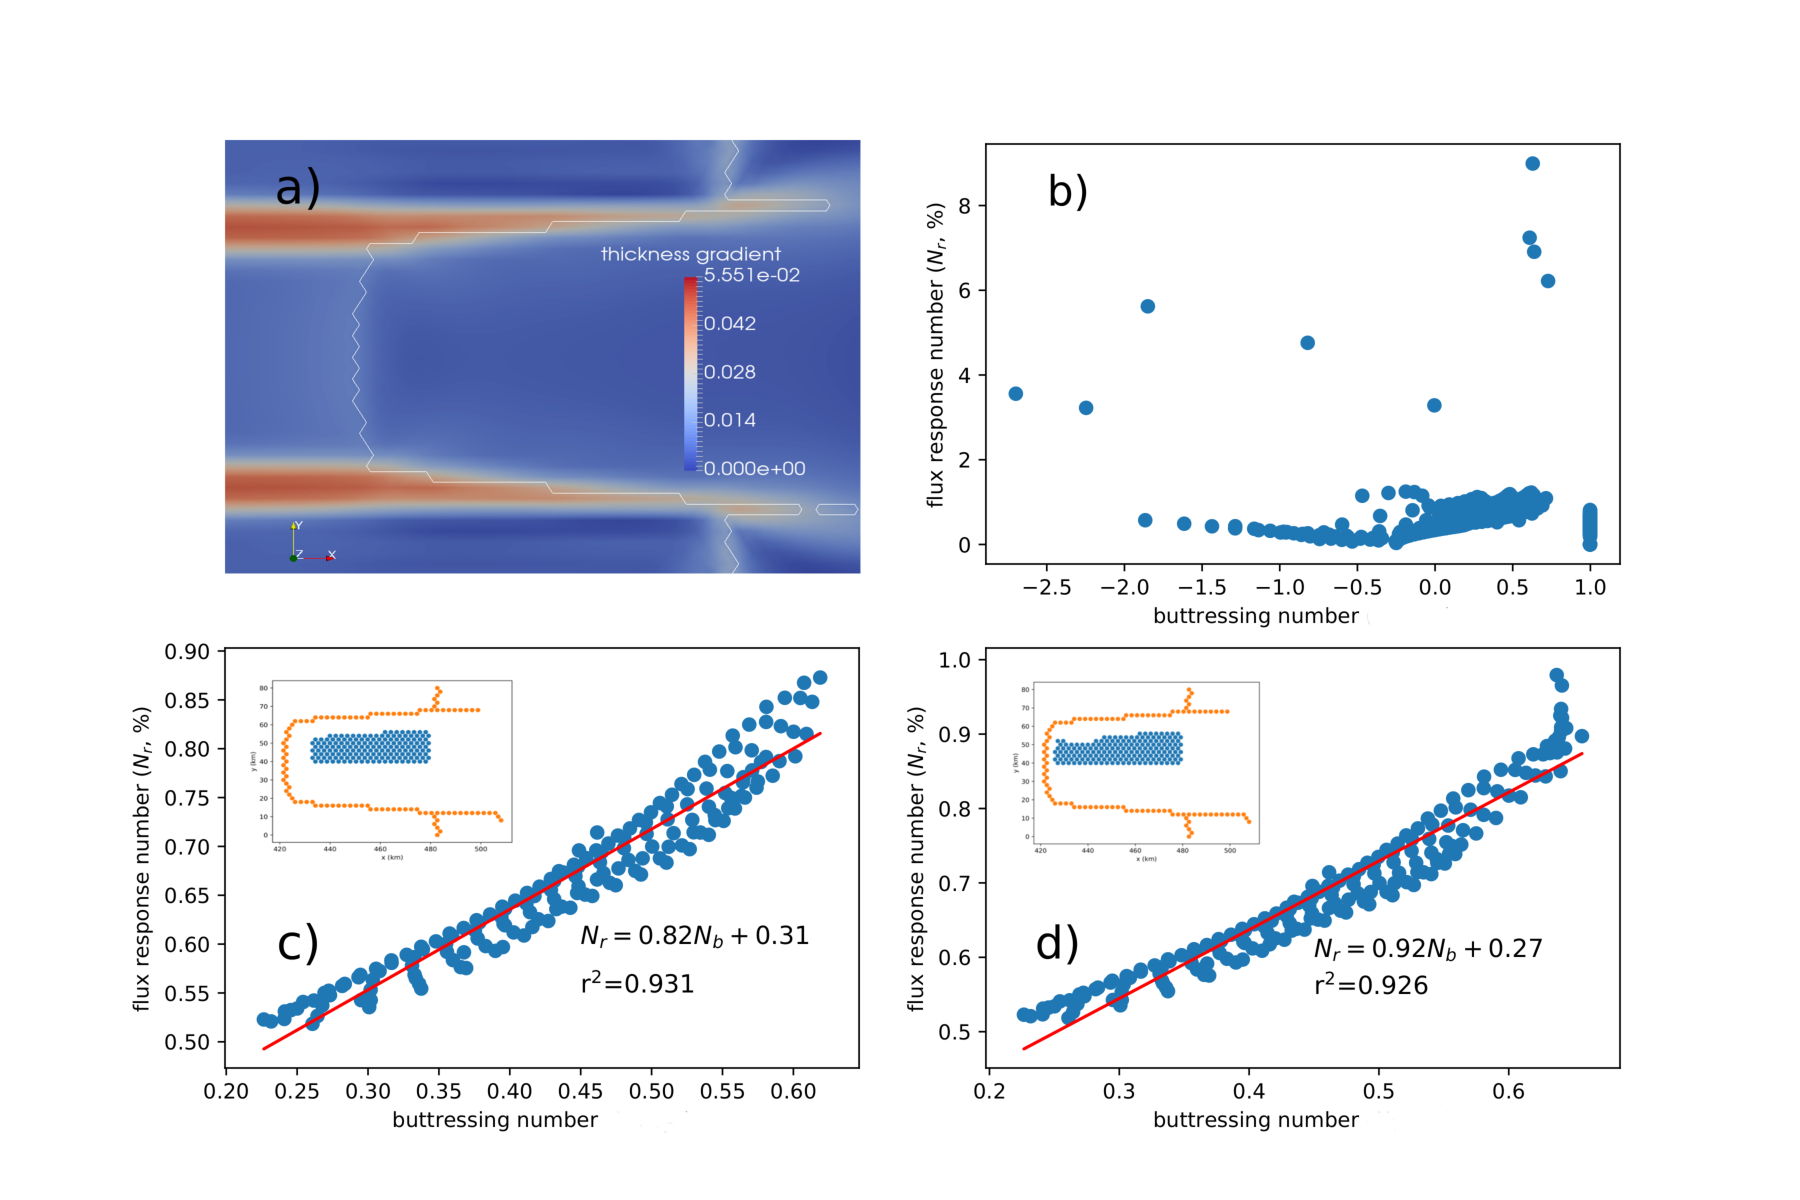
\includegraphics[width=1\linewidth]{figs/fig2.pdf}
    \caption{(a)MISMIP+ steady-state geometry. Color represents the magnitude of the ice thickness gradient and the white line represents the GL. (b) $N_b$-$N_r$ correlation for all perturbation points. (c) $N_b$-$N_r$ correlation for perturbation points satisfying $x>480$ and that are $>$10 km away from GL; (d) $N_b$-$N_r$ correlation for perturbation points satisfying $x>480$ and with a thickness gradient magnitude of $<7$x$10^{-3}$. In (c) and (d), the red (blue) dots in the insets represent the GL (perturbation) grid cells.}
\label{fig2}
\end{figure}

%\subsection{The buttressing directions}
\subsection{Correlation dependence on buttressing direction}

According to Equation \ref{butN}, the buttressing number $N_b$ is computed using the normal stress ($\sigma_{nn}$) along a specified direction. Therefore, the buttressing number at any perturbation point can vary depending on the chosen direction. \cite{furst2016} calculated $N_b$ along two directions, the ice flow direction and the direction corresponding to the second principle stress ($\sigma_{p2}$), and found that the latter -- the direction corresponding to the maximum compressive stress (or the least extensional stress) -- has the maximum impact on the ``passive'' ice shelf regions. In Figure \ref{fig3}, we plot the correlation coefficients ($r^2$) between $N_r$ and $N_b$ using values for $\sigma_{nn}$ that vary continuously by an angle $\Delta \phi$, between 0 and 180 degrees, relative to the direction of $\sigma_{p1}$. We find the largest correlation coefficient ($r^2>0.9$) when $N_b$ is aligned with the $\sigma_{p1}$ direction ($\Delta \phi=0^\circ$) and the smallest correlation coefficient ($r^2<0.4$) when $N_b$ is aligned with the $\sigma_{p2}$ direction ($\Delta \phi=90^\circ$). 
% for different directions with respect to the first principle stress and flow direction, respectively (Fig \ref{fig3}). Differently, we find that $N_b$ along the $\sigma_{p1}$ direction shows the best regression performance, whereas the $\sigma_{p2}$ appears to show the weakest correlations to $N_r$. This can be further testified by looking at the angle differences between $\sigma_{p1}$ and flow directions ($\Delta \phi = \phi_{flow}-\phi_{\sigma_{p1}}$). 

% As a second, somewhat independent check on the strong correlation between $N_r$ and $N_b$ as a function of the direction $\sigma_{p1}$, we also calculate the correlation coefficient for $N_b$ where the value for $\sigma_{nn}$ is calculated as a function of the ice flow direction. The blue line in Figure \ref{fig3}a is analogous to the red line but for the case where $\Delta \phi$ is relative to the ice flow direction. A similar sinusoidal pattern is evident, but with a phase lag of approximately $50^\circ$ relative to the red line. Thus, aligning the blue curve so that its maximum and minimum coincide with those of the red curve requires rotating the direction for calculating $\sigma_{nn}$ by $50^\circ$.    

This can be further testified by looking at the angle differences between $\sigma_{p1}$ and flow directions ($\Delta \phi = \phi_{flow}-\phi_{\sigma_{p1}}$). From Figure \ref{fig3}b, we see that for around 50\% of the perturbation points, their flow directions are around 30--50 degree more than the $\sigma_{p1}$ directions, which is consistent with the phase differences in Figure \ref{fig3}a. If we add around 40 degree on top of the flow direction (blue curve), the new direction will be likely aligned closely with the $\sigma_{p2}$ direction, which is consequently pointing to the smallest $r^2$ number for the $\sigma_{p1}$ (red) curve. This indicates that the local maximum buttressing relating to $\sigma_{p2}$ is unnecessarily corresponding to the integrated instantaneous GLF responses. (\textbf{SP: I tried to reword this so that it is a bit more clear, but I failed (commented out my new version of it). I'm going to leave it for the time being and come back to it later. But I also wonder if this discussion is necessary or if it is just too confusing.})

In the following sections, we elaborate our understandings of the dependence on buttressing directions.

\begin{figure}
\centering
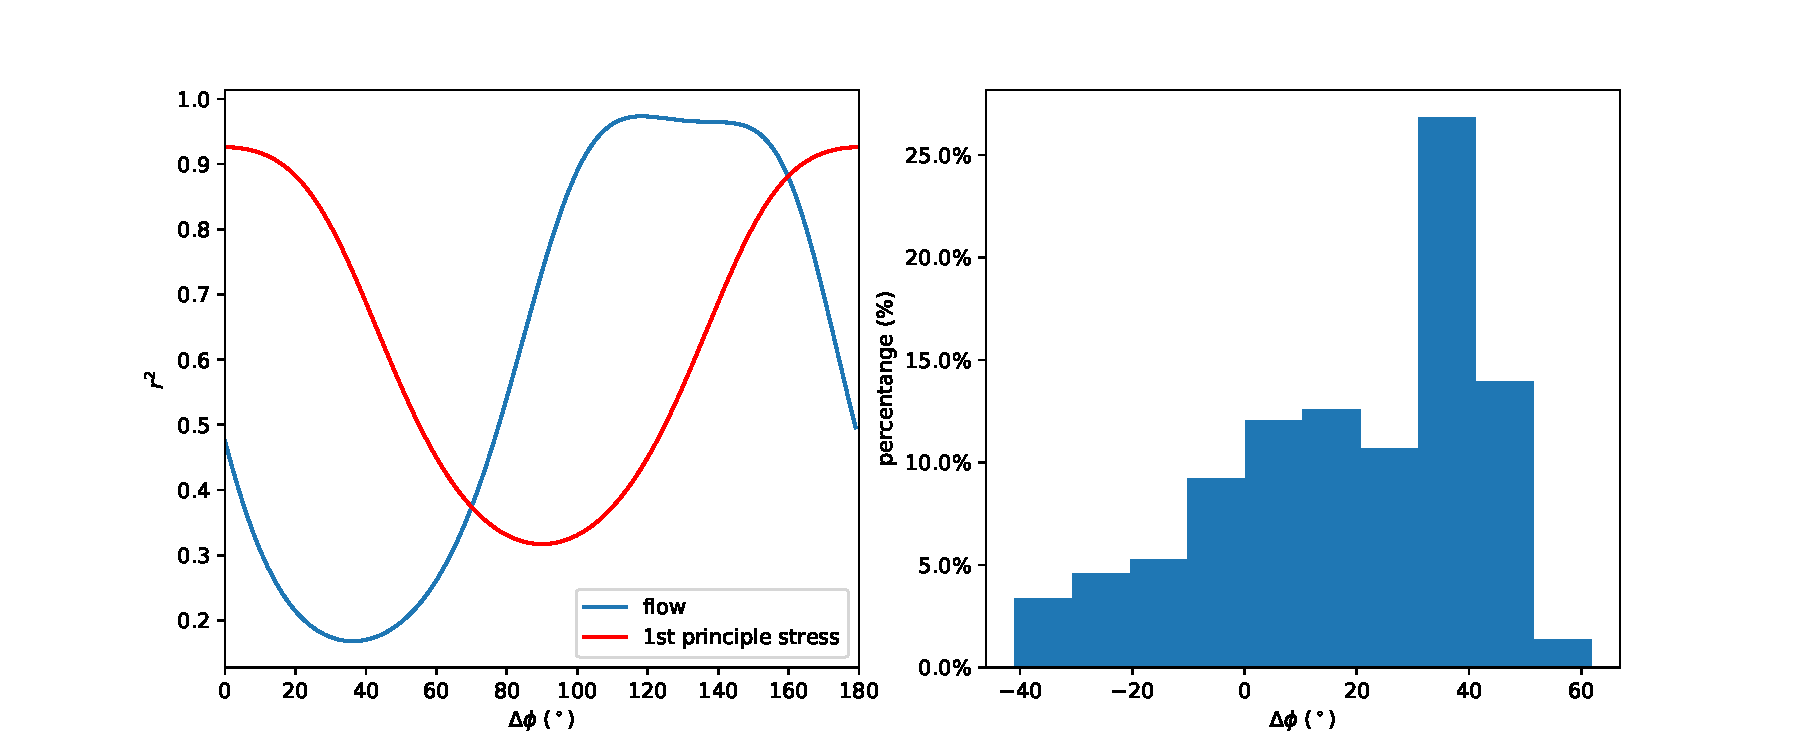
\includegraphics[width=1\linewidth]{figs/fig3.pdf}
    \caption{(a) $N_b$-$N_r$ correlation coefficients for $\sigma_{nn}$ values rotated anti-clockwise by $\Delta\phi$ degrees relative to the $\sigma_{p1}$ direction (red)and the ice flow direction (blue). (b) Histogram of the angular differences between the flow direction and $\sigma_{p1}$ directions. The perturbation points analyzed here are those shown in Figure \ref{fig2}d.}
    \label{fig3}
\end{figure}

%\subsection{Possible controlling factors}
%\subsection{Understanding the dependence on buttressing direction}
\subsection{The changes of velocity around the perturbation spot}

The strong correlation between changes in GLF and the first principle stress can be understood by examining the spatial patterns of velocity change\footnote{In this case, velocity changes are a proxy for flux changes since ice thickness is changed only at the perturbation level.} and stress change associated with thickness perturbations. %Further clues of the impacts from different chosen directions can be found in Figure \ref{fig4}. 
In Figure \ref{fig4}, we plot histograms of the maximum (red) and minimum (blue) velocity changes as a function of angular distance (??) around each perturbation point for the case where $\sigma_{nn}$ is calculated along the ice flow direction or along the $\sigma_{p1}$ direction. Figures \ref{fig4}a and b include all perturbation points while Figures \ref{fig4}c and d contain only the points from Figure \ref{fig2}d (i.e., filtered according to ice thickness gradient). For $\sigma_{nn}$ calculated along the ice flow direction (Fig \ref{fig4}a,b), the maximum velocity changes cluster around the flow direction, while the minimum velocity changes cluster around 120 degrees to the flow direction. For $\sigma_{nn}$ calcualted along the $\sigma_{p1}$ direction (Fig \ref{fig4}c,d), the maximum velocity changes cluster between 0 and 45 degrees of the $\sigma_{p1}$ direction and the minimum velocity changes cluster between 90 and 120 degrees. From this analysis, it is clear that most of the maximum (minimum) velocity changes are aligned with the first (second) principle stress direction, supporting the hypothesis that the first principle stress direction is more important for \textit{... not sure how to close this yet. Something about how changes propagate more easily along p1 even though p2 ``controls'' the buttressing? Not sure we entirely understand this yet but we need to}.

\begin{figure}
	\centering
    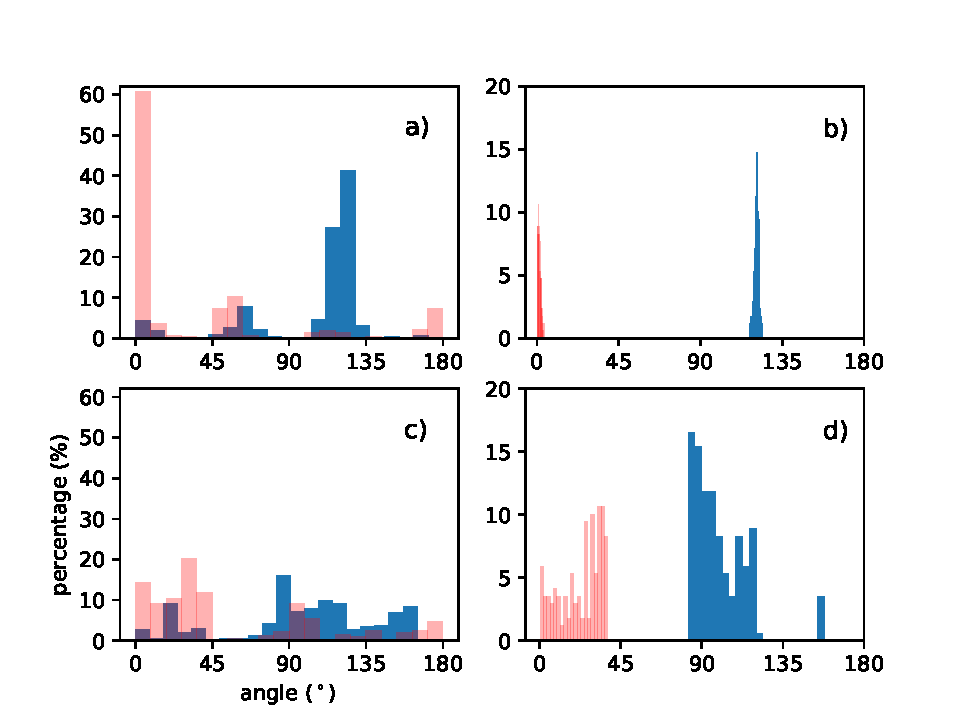
\includegraphics[width=1\linewidth]{figs/fig4.pdf}
    \caption{Histograms for the frequency of the maximum (red) and minimum (blue) velocity changes in neighboring grid cells as a function of angular distance around each perturbation point. In a and c, all perturbation points are shown and in plots b and d, only the subset of points from Figure \ref{fig2}d (b and d) are shown. ({\bf{TZ: this figure still needs double check!}})}
	\label{fig4}
\end{figure}

\subsection{The changes of velocity and stress along GL}

Further evidence for the importance of the first principle stress direction is given by the variances that characterize the changes in the state of stress and the state of velocity between the initial condition and the perturbation experiments. To this end, we define the metric $\Upsilon$,  
\begin{equation}
    \Upsilon= corr\left(\frac{\sigma_{p}-\sigma_{c}}{\sigma_{c}}, \frac{u_{p}-u_{c}}{u_{c}}\right),
\label{upsilon}
\end{equation}

%\begin{equation}
%    \Psi= \frac{\sigma_{p}-\sigma_{c}}{\sigma_{c}}-\frac{u_{p}-u_{c}}{u_{c}},
%\label{psi}
%\end{equation}
where the subscripts $p$ and $c$ denote the perturbation experiments and the ``control'' (i.e., the initial condition), respectively, and $\sigma$ and $u$ denote the stress component and ice velocity, respectively. Here the changes of $\Upsilon$ we discuss is limited to GL. $\Upsilon$ are a measure of the consistency between changes in the model stress and velocity states between the control (the initial condition) and perturbation experiments. We calculate $\Upsilon$ for every perturbation point for each direction from 0--180$^\circ$ (Figure \ref{stress_vel_corr_GL_allP}). Clearly, when we pick the $\sigma_{p1}$ direction as the buttressing direction, we can find the best correlation between the changes of ice surface speed and normal stress along GL, whereas the correlation numbers are relatively low when the buttressing directions are close to the $\sigma_{p2}$ direction.  
\begin{figure}
	\centering
    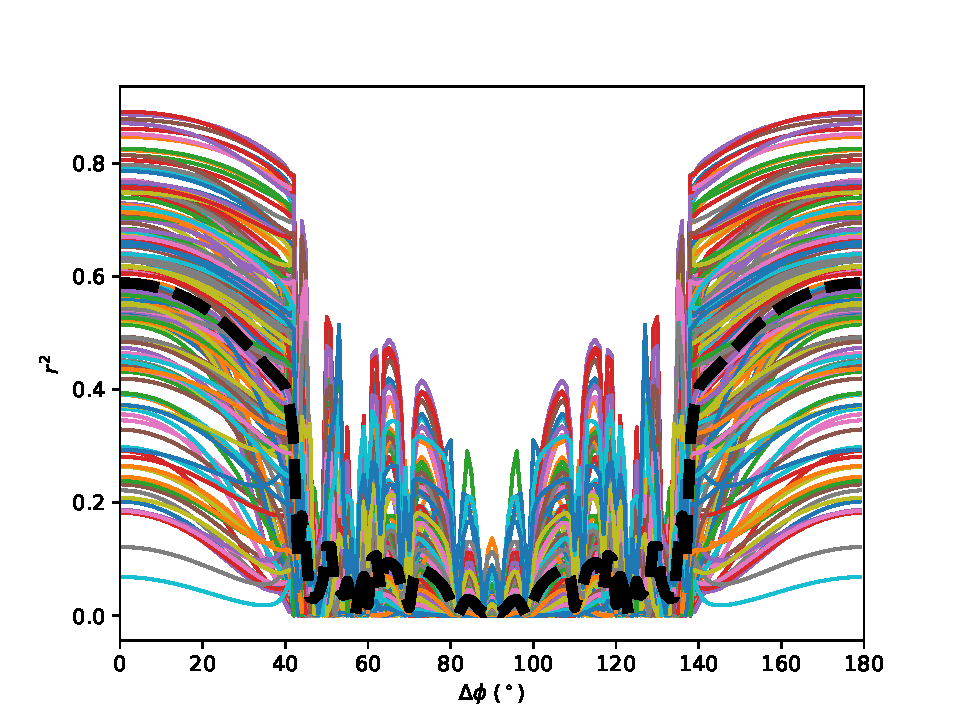
\includegraphics[width=1\linewidth]{figs/stress_vel_corr_GL_allP.pdf}
    \caption{The correlation ($\Upsilon$) between the changes of ice surface speed and the changes of normal stress along GL. The direction of normal stress is rotated anti-clockwisely from the direction of $\sigma_{p1}$. Each colored curve represents a perturbation experiment, and the thick dashed back curve is their mean value.}
	\label{stress_vel_corr_GL_allP}
\end{figure}

More specifically, we can see the spatial pattern of $\Upsilon$ for every perturbation point for the case where $\sigma_{nn}$ in Equation \ref{butN} is set equal to $\sigma_{p1}$ (Fig \ref{fig5}a) and $\sigma_{p2}$ (Fig \ref{fig5}b). From Figure \ref{fig5}, it is clear that the correlation between stress and velocity change along GL is generally much larger in the domain for the case of $\sigma_{nn}=\sigma_{p1}$, especially for some regions in the center of the domain. \textit{SP: Or something like this. Need to think about it some more still. I wonder if it could also be interpreted differently -- e.g., in 5b, could the much larger variance be because a small change in p2 results in a much larger change in velocity (relative to p1)?. Would it make more sense for Fig. 5 to be an actual correlation coeff. plot rather than the somewhat complicated variance comparison?}. \textbf{TZ: I now change deviation to correlation. You are right. It's more consistent. I think the problem is to check if the changes of $\sigma_{p1}$ or $\sigma_{p2}$ can cause more consistent velocity changes along GL, right? For example, if $\sigma_{p2}$ can cause a larger but more consistent change in vel. than $\sigma_{p1}$, then $\sigma_{p2}$ is still the better metric than $\sigma_{p1}$.} In Figure \ref{fig6} we show the stress and velocity changes at the GL for a perturbation at a specific location on the ice shelf, which may provide a more clear evidence of a strong (weak) correlation between changes in the first principle stress (second principle stress) and changes in the velocity (Figure \ref{fig6}). For this particular perturbation spot, we can also see the changes of buttressing number calculated by $\sigma_{p1}$ (Figure \ref{sigma_change_example}a) and $\sigma_{p2}$ (Figure \ref{sigma_change_example}b) across the domain. In this case the buttressing number calculated from $\sigma_{p1}$ shows more decrease than that from $\sigma_{p2}$ for most upstream parts to the perturbation spot, indicating another evidence that the more tensile stress $\sigma_{p1}$ can change more significantly and therefore contribute more to the changes of ice shelf buttressing under certain basal melt forcing scenarios. 

% This possibly indicates that GLF are more relevant to the changes of $\sigma_{p1}$ along GL, compared to the $\sigma_{p2}$ case, which can be clearly found if we look at some specific perturbation example as shown in Figure \ref{fig6}. 

\begin{figure}
	\centering
    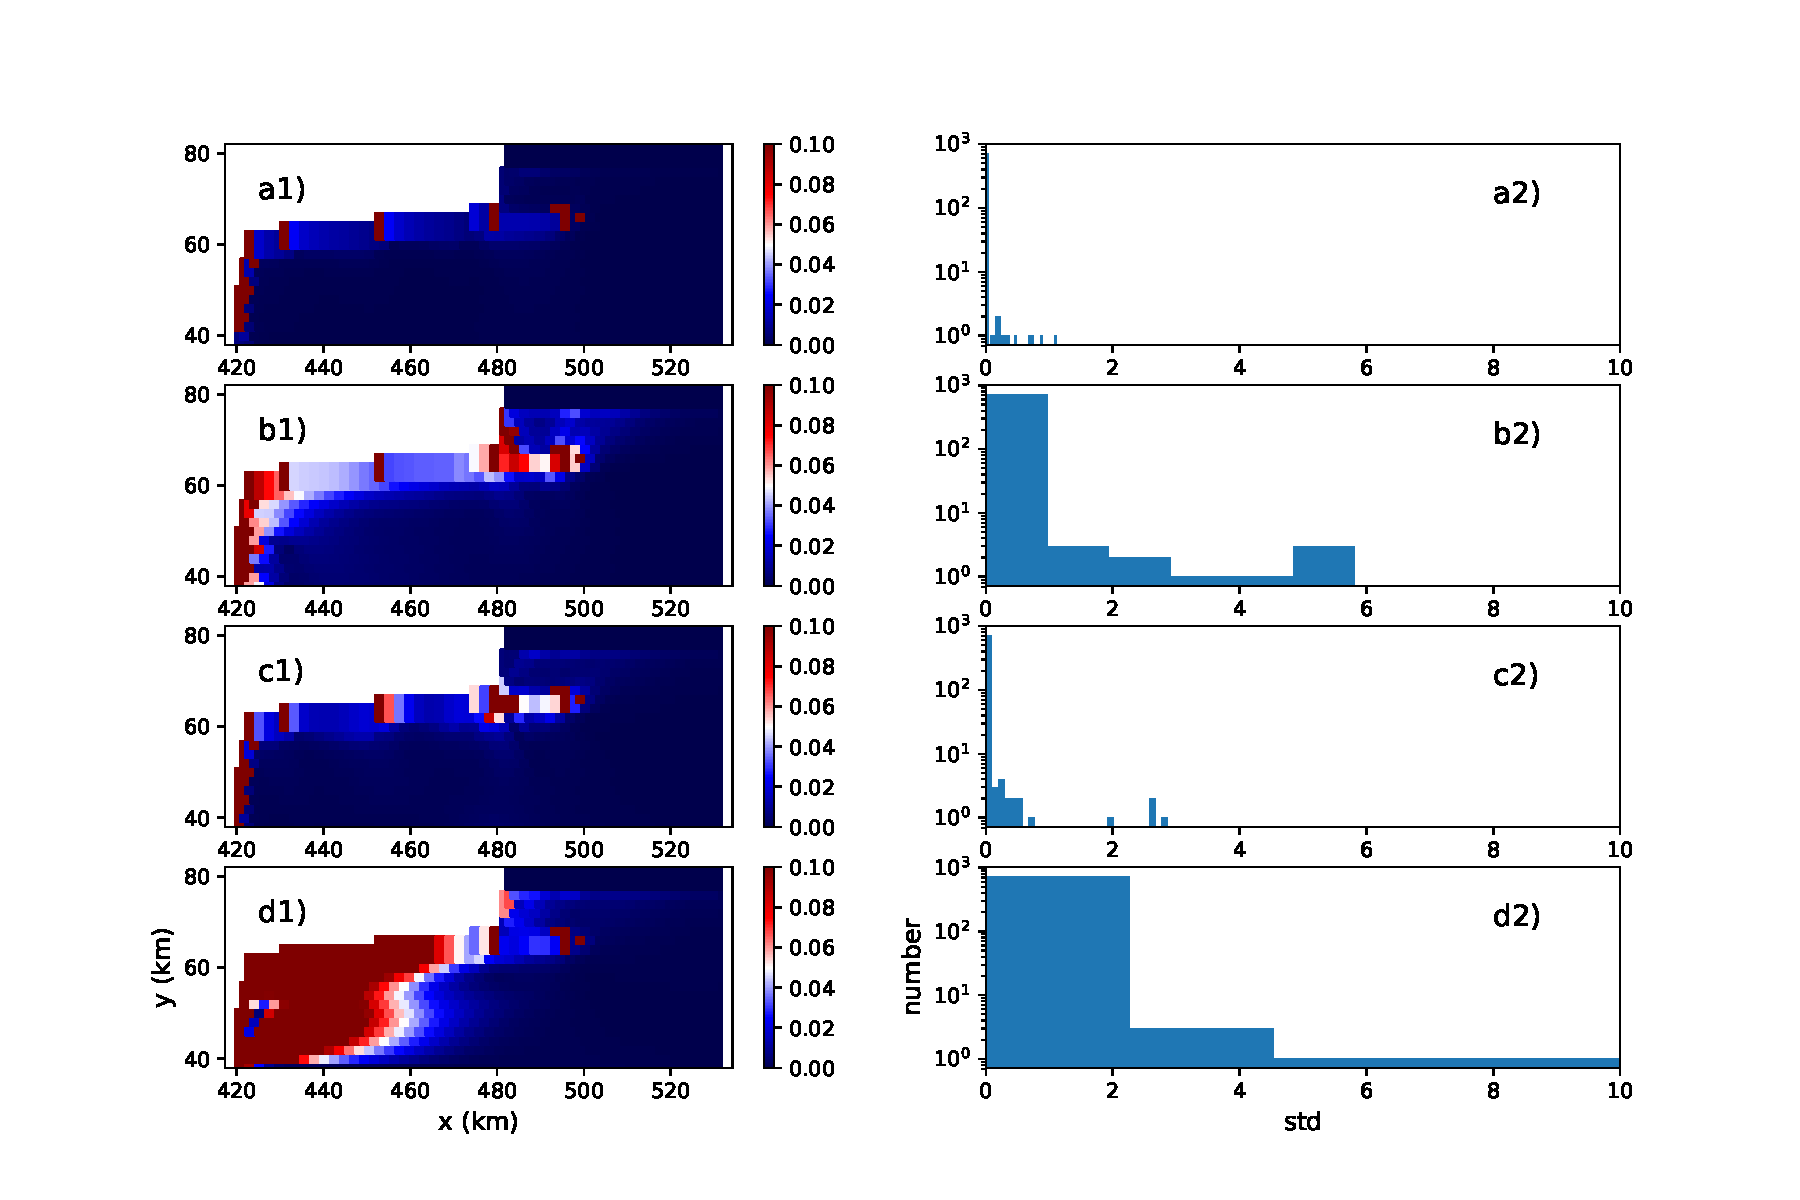
\includegraphics[width=1\linewidth]{figs/stressDiff_velDiff_GL_allPerturb.pdf}
    \caption{The standard deviations of $\Psi$ -- a metric for how closely a change in normal stress corresponds with a change in velocity -- at each perturbation point of the MISMIP+ domain, for the case of $\sigma_{nn}=\sigma_{p1}$ (a) and $\sigma_{nn}=\sigma_{p2}$ (b).}
	\label{fig5}
\end{figure}

\textit{SP: Leaving this section alone for now. I think it's worth including some additional discussion here if we can make some reasonable speculation as to what's going on \textbf{TZ: The metric regarding distance and flow/stress angle is a such speculation that the impact of perturbation on GLF is a combined effect of perturbation and GL dynamics (see below)}. But we probably need to come up with a bit more than this. I wonder if there are other T3 folks who might have some insight into this problem \textbf{TZ: there might be some similar theory going on here, but I doubt the pure mechanical knowledge apply in this specific problem. Perhaps Xylar can contribute a bit from the perspective of Fourier transform theory} ? One thing that occurs to me is that we could be conflating cause and effect here. For example, when we look at Figure 6, it looks like the changes in velocity correlate with changes in $\sigma_{p1}$, whereas they don't correlate with changes in $\sigma_{p2}$. But it could simply be that the changes in $\sigma_{p2}$ (due to the thickness perturbation) are causing a velocity change, and the velocity change is better reflected by the change in $\sigma_{p1}$. This makes sense at the GL, where we know the velocity / flux are largely going to be aligned with the $\sigma_{p1}$ direction (perpendicular to the GL). This doesn't, however, explain why we see a good correlation between changes in velocity / flux at the GL (reflected by the flux response number, N) and $\sigma_{p1}$ but a much poorer correlation between the flux response number and $\sigma_{p2}$. \textbf{TZ: I am not sure if I follow you here. I don't know if it's a proper way to say that the changes in $\sigma_{p2}$ cause the changes in velocity. If we look closely at Figure \ref{fig6} we can see that for some cells on GL, even though the velocity direction is more aligned with p1, the correlation is still poor, whereas the correlation with p2 is better for these same cells. The difference here is their respective angle difference with the stress direction at perturbation spot (a main reason I make up the metric in the following; I can show you some point when you have time). It's hard to know exactly the reason behind.}} One of the possible reasons for us seeing such direction-dependent correlations might be due to the perturbation propagation features on ice shelves. The energy of perturbation propagates with the group velocity if we decompose it using Fourier transform. A similar example can be found in \citep{gudmundsson2003}. Using very simplified geometry \cite{gudmundsson2003} analyzed the propagation of basal perturbation to glacier surface and found that the direction of group velocity is aligned closely with the main flow. The existence of preferred propagation direction for the perturbations can possibly lead to our findings that favor the first principle stresses (\textbf{TZ: I am still not able to explain why it's exactly the first principle stress direction :(}). 

\begin{figure}
	\centering
    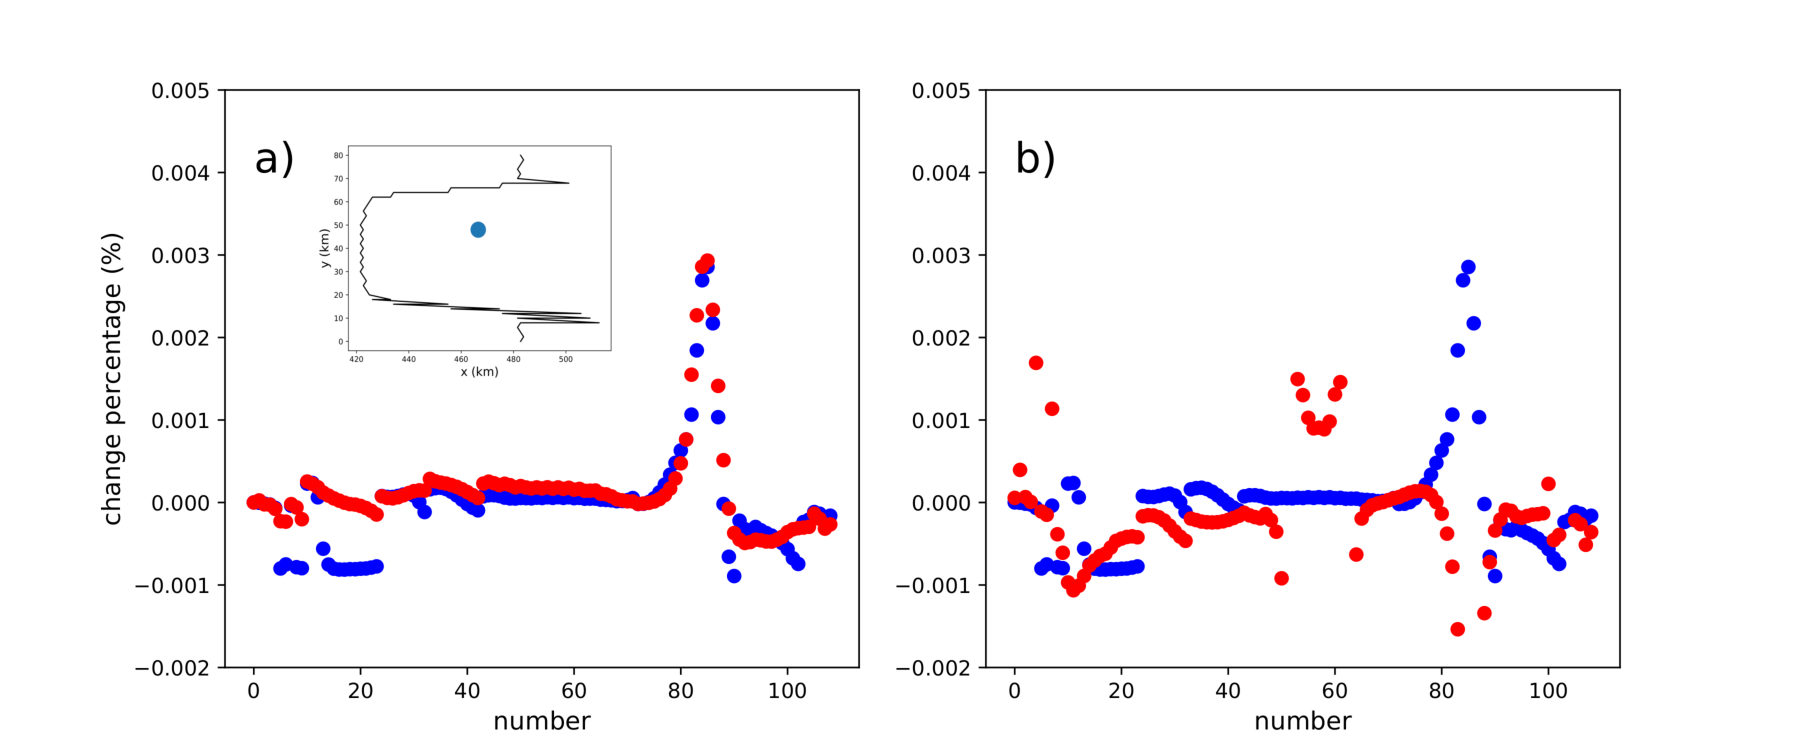
\includegraphics[width=1\linewidth]{figs/fig6_new.pdf}
    \caption{Relationship between GL {changes} in the velocity (blue) and in the stress (red) for the MISMIP+ test case due to a perturbation at a specific location on the ice shelf (blue dot in inset map). In a), changes in GL velocity are plotted against changes in $\sigma_{p1}$ and in b) changes in GL velocity are plotted against changes in $\sigma_{p2}$. The $x$-axis is an index for the grid cell number along the GL.}
	\label{fig6}
\end{figure}

\begin{figure}
	\centering
    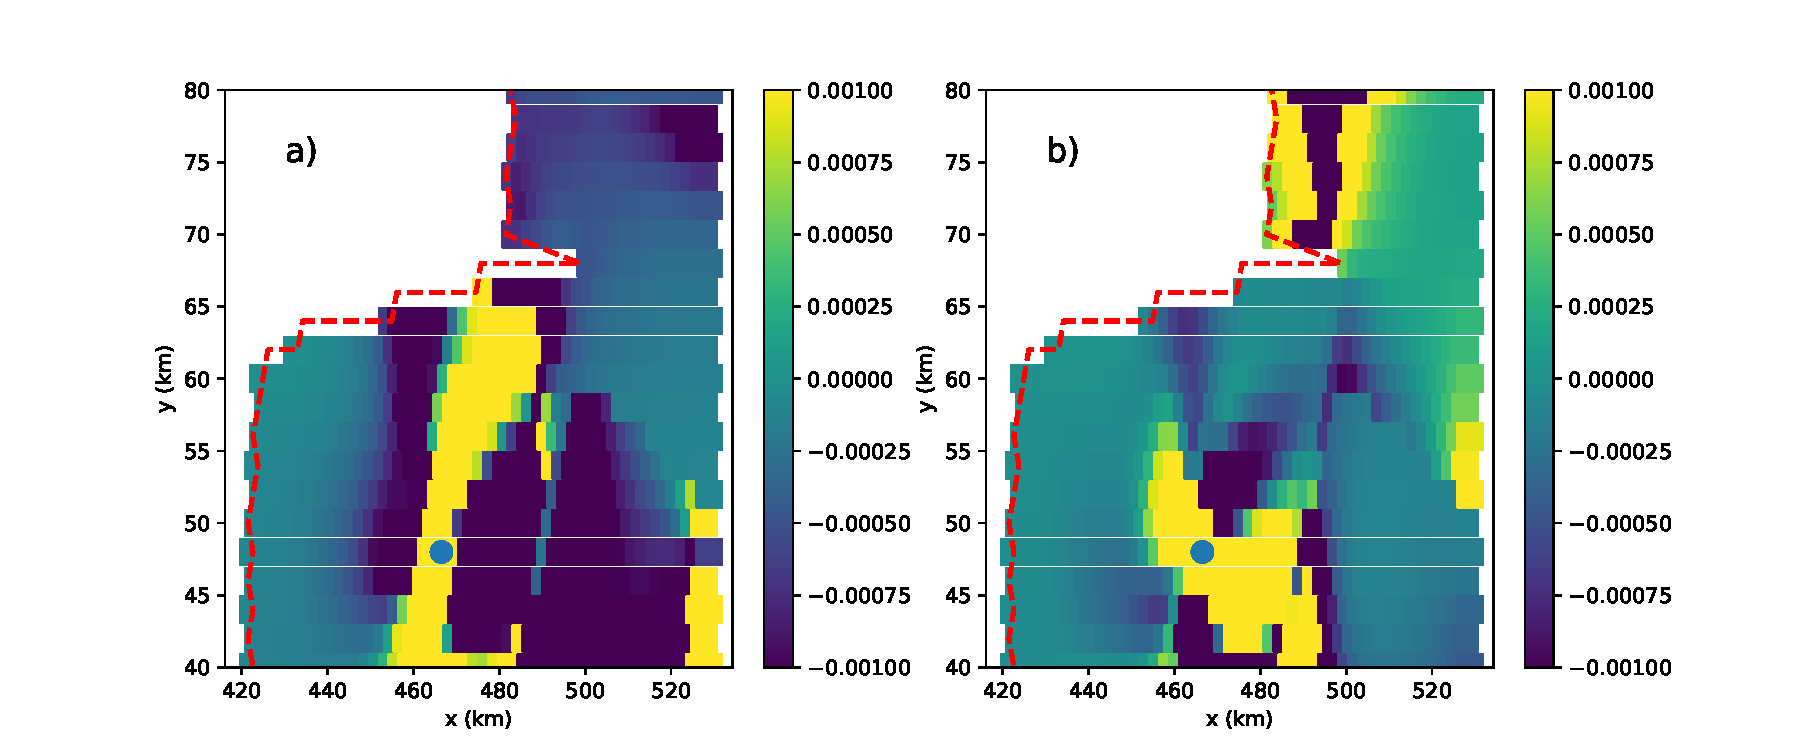
\includegraphics[width=1\linewidth]{figs/sigma_change_example.pdf}
    \caption{Relationship between GL {changes} in the velocity (blue) and in the stress (red) for the MISMIP+ test case due to a perturbation at a specific location on the ice shelf (blue dot in inset map). In a), changes in GL velocity are plotted against changes in $\sigma_{p1}$ and in b) changes in GL velocity are plotted against changes in $\sigma_{p2}$. The $x$-axis is an index for the grid cell number along the GL.}
	\label{sigma_change_example}
\end{figure}

\subsection{A possible metric connecting perturbation and GLF}

The propagation of perturbation is likely determined by the flow regime on the ice shelf, i.e., the change of GLF is controlled by both the perturbation (geometry, stress field) and its surrounding ice dynamic features. To verify this we make the following metric:

\begin{equation}
    \Lambda = \sum_i^I \frac{1}{d_i} |\mathrm{cos} \left(\theta_i\right)|,
    \label{Lambda}
\end{equation}
where $I$ is the total cell number on GL, $d_i$ is the distance between the perturbation spot and the $i$-th cell on GL, $theta_i$ is the angle difference between the direction of the specified normal stress at the perturbation spot and the flow direction for the $i$-th cell on GL. This metric gives us two possible important factors that impact GLF: 1) the geometric location of perturbation spot(the closer perturbation spots to GL, the larger impact of perturbation on GLF; see the discussion in the following section ``Impacts of near-GL perturbations''), 2) the relationship between ice flow along GL and the buttressing direction we choose at the perturbation spot (the perturbation has more impacts on GLF if the buttressing direction aligned more closely with the ice flow directions on GL).  
Similar to above, we rotate the buttressing direction by 1--180$^\circ$ on top of the $\sigma_{p1}$ direction, and calculate $\Lambda$ for each perturbation spot. From Figure \ref{new_metric_new} we can see that $\Lambda$ has large values when the buttressing directions are close to the $\sigma_{p1}$ direction ($\Delta\phi=0^\circ$ or $\Delta\phi=180^\circ$). This is because, for MISMIP+, the $\sigma+{p1}$ on GL largely controls the GLF (see the quiver plots of principle stresses in the Appendix). For real ice shelves, the pattern of ice flow along GL might be much more complex then of MISMIP+m, resulting in difficulty of predicting GLF using single direction buttressing number.  


\begin{figure}
	\centering
    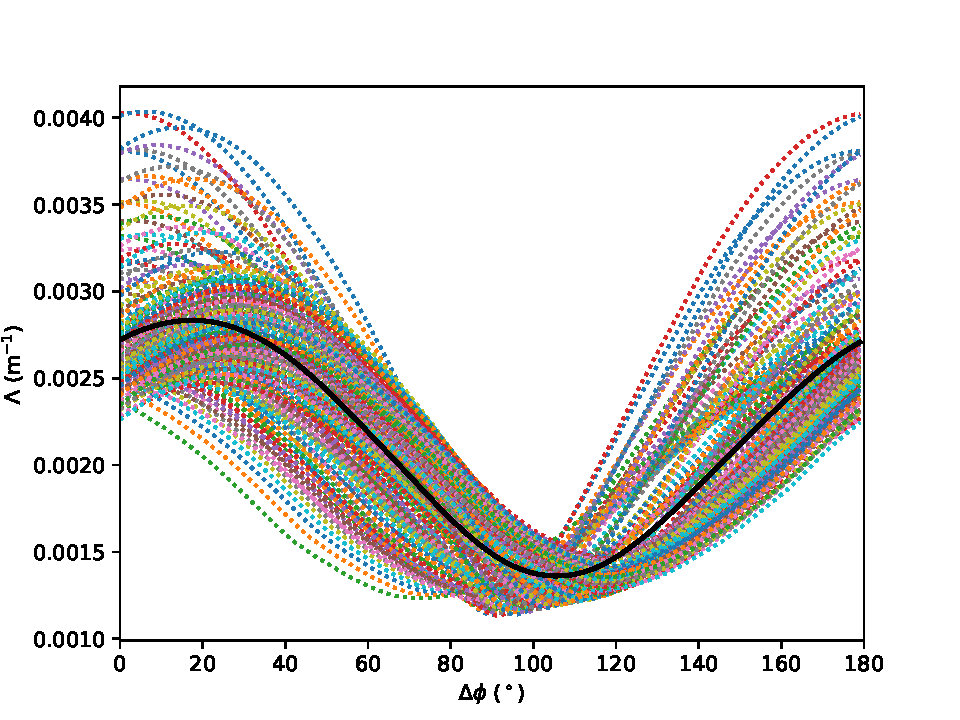
\includegraphics[width=1\linewidth]{figs/new_metric_new.pdf}
    \caption{The standard deviations of $\Psi$ -- a metric for how closely a change in normal stress corresponds with a change in velocity -- at each perturbation point of the MISMIP+ domain, for the case of $\sigma_{nn}=\sigma_{p1}$ (a) and $\sigma_{nn}=\sigma_{p2}$ (b).}
	\label{new_metric_new}
\end{figure}


\subsection{Application to Larsen C ice shelf}

To explore whether the correlations between $N_b$-$N_r$ for the MISMIP+ test case hold for realistic ice shelves, we apply a similar analysis to our Larsen C domain. In this case, the computational mesh resolution varies, from finer near the GL (xx km) to coarser towards the center of the ice shelf and calving front (yy km). We use 20 km $\times$ 20 km boxes for the application of ice thickness perturbations (as in \citet{reese2018}) where the number of grid cells contained within each perturbation ``box'' is adjusted in order to sum to the correct area. Additionally, to account for the complex geometry of the Larsen C ice shelf (i.e., the GL shape, the existence of ice rises, etc.), we apply two different sets of perturbation experiments, both with and without perturbations applied to boxes containing the GL. % for investigating further the nonlinearity feature we observe in the above MISMIP+ section. 

Analagous to Figures \ref{fig3}a,b for the MISMIP+ test case, Figures \ref{fig7}a,b shows the correlations between $N_b$ and $N_r$ for the Larsen C model domain. As previously, calculating $N_b$ using $\sigma_{nn}=\sigma_{p1}$ provides the best overall correlation between $N_b$ and $N_r$ (red curve for $\Delta\phi=0^\circ$) and calculating $N_b$ using $\sigma_{nn}=\sigma_{p2}$ provides the worst overall correlation (red curve for $\Delta\phi=90^\circ$). \textbf{SP: As noted above, I'm not sure about introducing the discussion about results relative to the velocity direction, as I think they are maybe just confusing. So leaving this next part alone for now.} The phase difference between the $\sigma_{p1}$ and flow direction results can also be partially explained by their respective angle differences. In Figure \ref{fig7}b we can find the angles of flow directions are mostly around 90--100 degrees larger than that of the $\sigma_{p1}$ directions. This is a bit biased than the around 70 degree difference in Figure \ref{fig7}a. However, considering the stress values (and thus $N_b$) for each perturbation box are averaged over multiple cells, we argue this difference is probably an acceptable error during our calculation.  

In Figures \ref{fig7}c, d we include points near to the GL in the analysis, which 1) reduces the $r^2$ values and 2) changes the relationship between the correlation coefficients and the direction aligned with $\sigma_{p1}$. Specifically, while the direction aligned with $\sigma_{p2}$ still gives the worst correlation between $N_b$ and $N_r$, the direction giving the best correlation is rotated by approximately $40^\circ$ relative the direction associated with $\sigma_{p1}$. \textit{SP: I'm not really sure what else we can say about this, other than that it's an indication that using $\sigma_{p1}$ and $\sigma_{p2}$ in the calculation of $N_b$ is probably just more problematic for complex geometries.} 
%Although the angle differences between the flow and $\sigma_{p1}$ directions are still mostly near 90 degree, there are no longer clear patterns in the phase differences for the corresponding $r^2$ curves. In addition, the $\sigma_{p1}$ directions are also no longer indicating the best $r^2$ correlations. However, the directions along $\sigma_{p2}$ appears to still pointing to the weakest $N_b$-$N_r$ correlations, despite the overall much smaller $r^2$ values in this case.

\begin{figure}
	\centering
    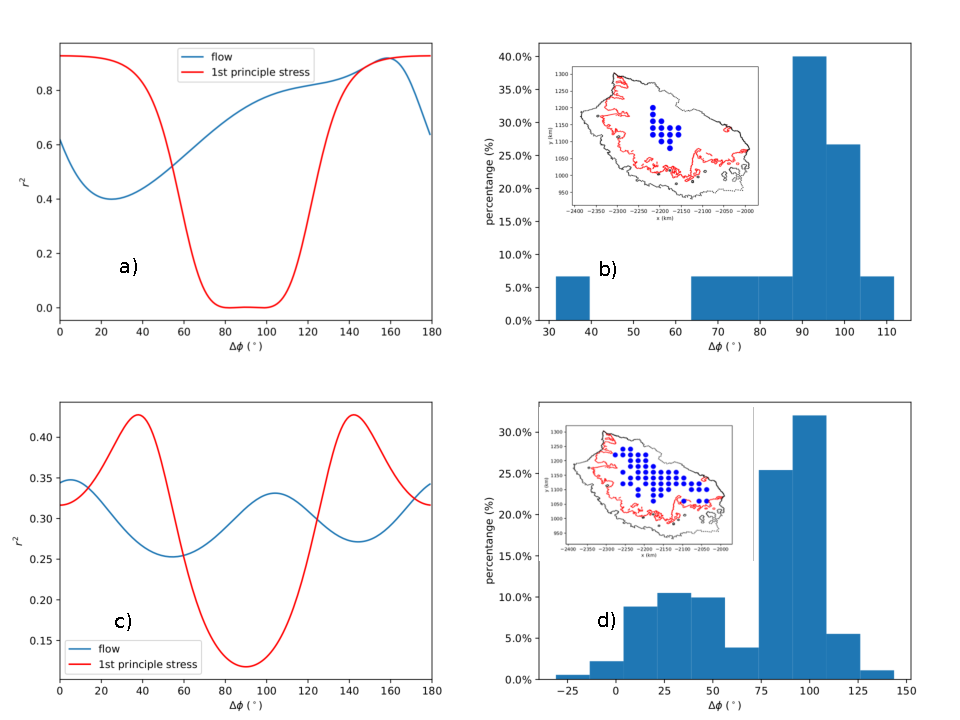
\includegraphics[width=1\linewidth]{figs/fig7_new.pdf}
    \caption{(a, c) The $N_b$-$N_r$ regression coefficients for each direction rotated anti-clock-wisely from the $\sigma_{p1}$ (red) and flow direction (blue); (b, d) The histogram of the angle differences between flow and $\sigma_{p1}$ directions. The insets in b) and d) show the perturbation boxes (blue circles).}
	\label{fig7}
\end{figure}

\subsection{Impacts of near-GL perturbations}
For the near-GL perturbations, it is hard to find similar linear regression relationship as discussed above. Alternatively, they are largely controlled by the distance between GL and perturbation points and also by the geometric features around them. As the perturbation decays over distance \citep{lick1970}, the neighboring GL cells of those near-GL perturbations will relatively easily detect the perturbation energy. This can be verified by looking at the standard deviations of GL velocity change due to each perturbation (Fig \ref{fig8}). For perturbations close to GL, their corresponding GL flux changes are in general confined to local regions, while in the remote GL sections the velocity changes are often negligible, resulting in large standard deviations. This can possibly cause spatial heterogeneity of GL retreating if the sub-shelf melting is very close to GL and is heavily local confined. 

The propagation of perturbation can also be impacted by the spatial GL geometry, e.g., they can be blocked by the local GL. For example, the perturbation at around x = 480 km and y = 65 km in Figure \ref{fig8}a can not directly impact the ice flow on the other side of the grounded peninsula (e.g., x=485 km, y=70km) in the same way as for it's neighboring cells. This is one of the major factors that complicate our diagnostic analysis for real ice shelves (for example, Larsen C) containing complex GL shapes and geometries. \textit{SP: Is there any way we could show this? E.g., for the Larsen C test case, could we plot the local GLF changes for a perturbation that is partly hidden behind an island / penn? We might actually be able to see the ``shadowing'' in the case. That is, we might be able to see that the portion of the GL that is blocked from a perturbation has a GLF that doesn't change much whereas nearby points along the GL that aren't block do change. I think this would just require plotting some maps from individual perturbation experiments for locations around some of these types of features.}
 
\begin{figure}
	\centering
    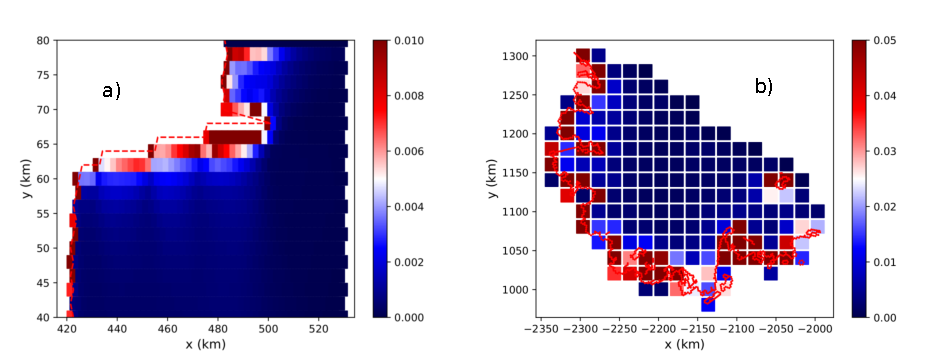
\includegraphics[width=1\linewidth]{figs/fig8.pdf}
    \caption{Standard deviation of velocity change along GL for each perturbation point for the MISMIP+ (a) and Larsen C (b) experiment. The red dashed lines (points) are the GLs for MISMIP+ (a) and Larsen C (b) .}
	\label{fig8}
\end{figure}

\subsection{Adjoint sensitivity}

Another altogether different approach to diagnosing the sensitivity of the flux across the grounding line to changes in ice shelf geometry is provided by the adjoint approach. This approach provides results analogous to those presented and discussed above but at a greatly reduced cost (and with improved accuracy?): rather than using the forward model to examine the sensitivity of GLF change to perturbations at each of \textit{n} model grid cells, a single adjoint solve is used to deduce those same sensitivities \textit{simultaneously} at all \textit{n} grid cells. 

\textit{SP: Will need Mauro to fill in some of the technical details here.}

In Figure \ref{fig9}, we provide a demonstration for the case of the MISMIP+ domain by comparing sensitivities deduced from X individual forward model evaluations (i.e., the perturbation experiments discussed above, and analagous to those in \citet{reese2018}) with those deduced from a single model adjoint solve. Here, the ``sensitivity'' is defined as BLAH. \textit{SP: need more information on techincal deatils here.} 

The comparison in Figure \ref{fig9} demonstrates that, for points in the domain we expect to be comparable, the two approaches provide a near exact match. While we cannot provide definitive proof, we suggest that the disagreement in sensitivity near the GL is likely a result of errors in the forward modeling approach, which prohibit us from controlling errors associated with the choice of a finite perturbation size (other reasons?).

\begin{figure}
	\centering
    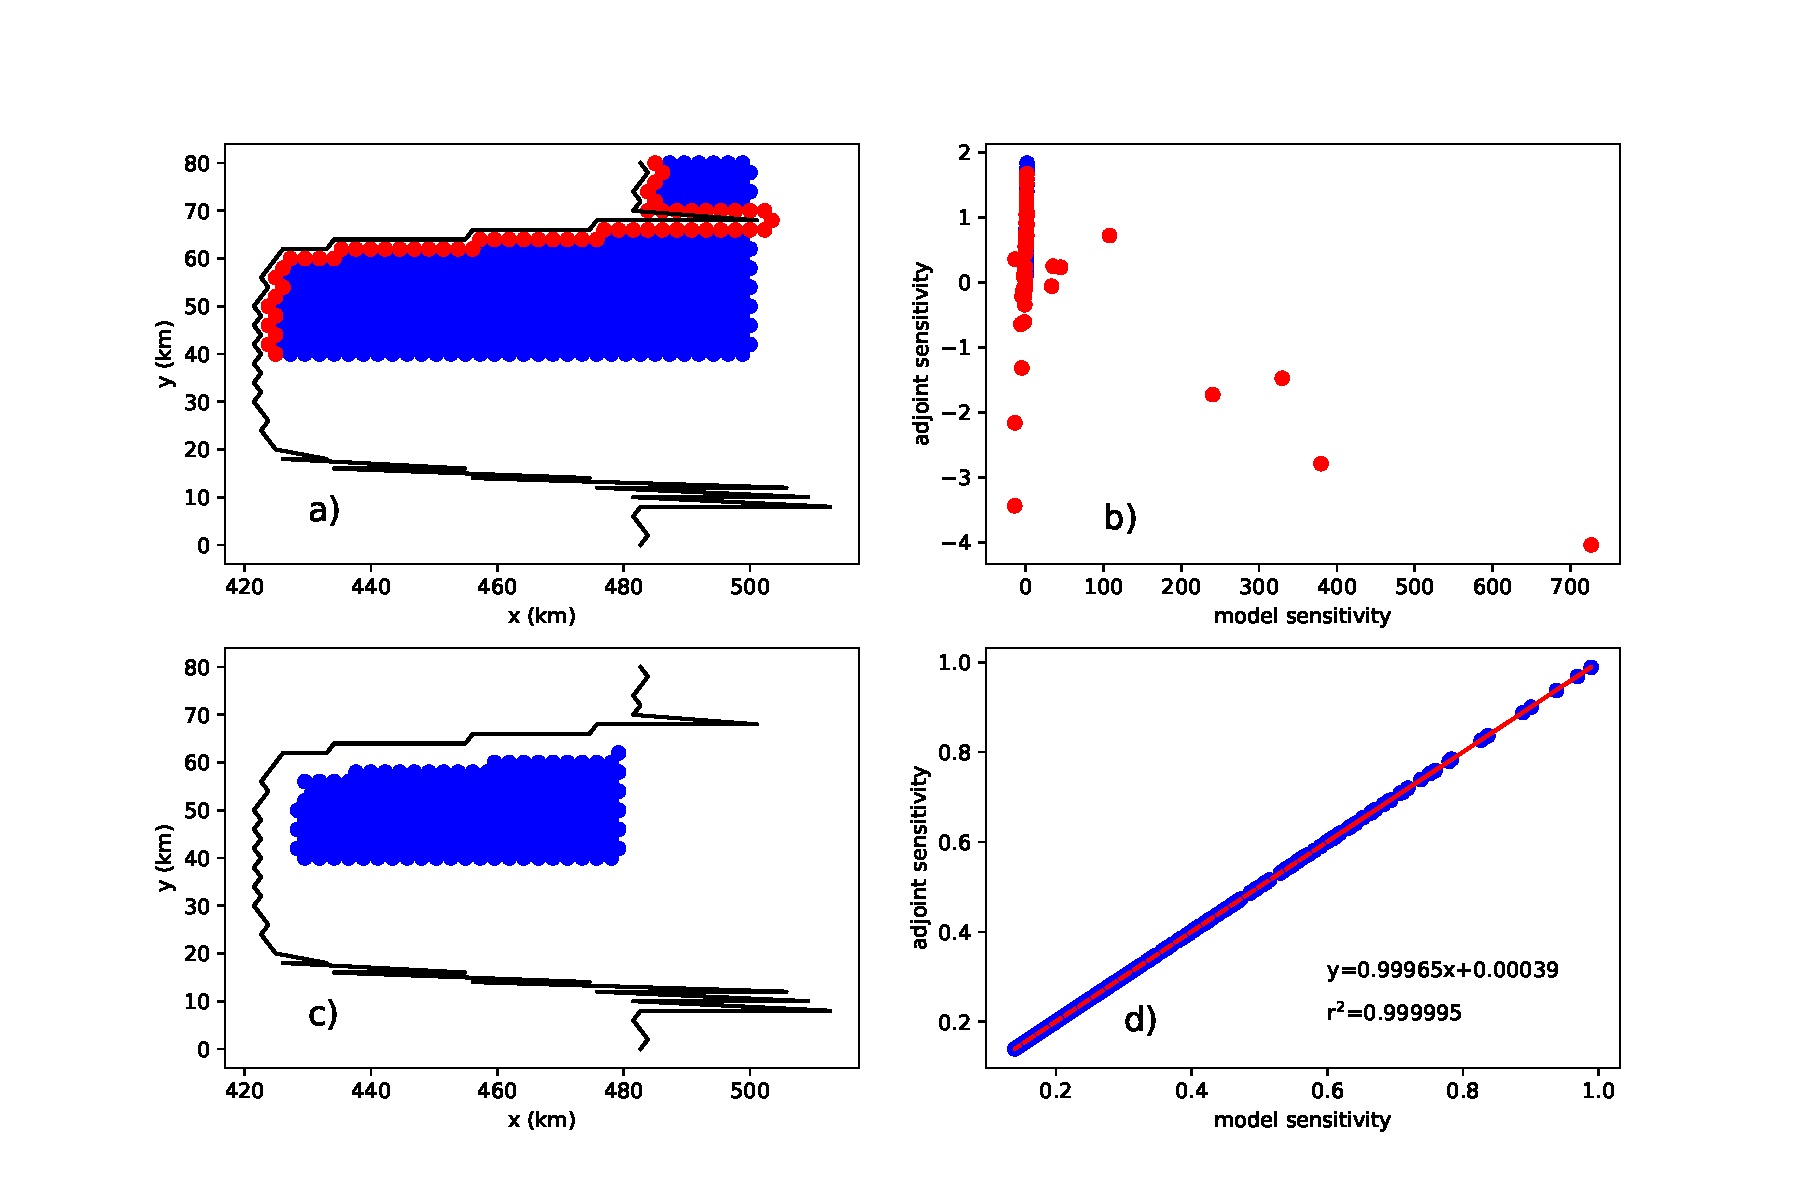
\includegraphics[width=1\linewidth]{figs/fig9.pdf}
    \caption{Grounding line flux sensitivity for the MISMIP+ domain calculated from individual perturbation experiments versus derived from a model adjoint (perturbation locations are shown by circles in a and c). Perturbation-experiment (x-axis) and adjoint-derived (y-axis) sensitivities (see text for definition) are plotted against one another in b and d. In a and b, the red circles indicate near-GL ($<$2 km) perturbation points, which are omitted in the comparison in b and d. The GL in a and c is shown by the black curve. In b and d, the red line is a linear regression between the perturbation-experiment and adjoint-derived sensitivities.}
	\label{fig9}
\end{figure}



%\subsection{MISMIP+}
%Before and after the perturbation, the GL velocity change clearly shows a spatial pattern (Fig \ref{stndVarFluxP}a). By calculating the standard deviation of the velocity change along GL for each 2 km perturbation experiment, we can see that the GL velocity change data is more dispersed for perturbation near GL, while for pertuirbations at the central region of the ice shelf, the corresponding GL velocity change is less variant along GL. If we look at Figure \ref{stndVarFluxP}b, the integrated GL flux is more contributed by the GL cells that close to the perturbation spot, i.e., the neighboring GL cells appears to have more flux contribution weight than those far away from the perperturbation location, and the perturbations near the ice shelf center tend to impact more uniformly on the GL dynamics.

%\begin{figure}
%\centering
%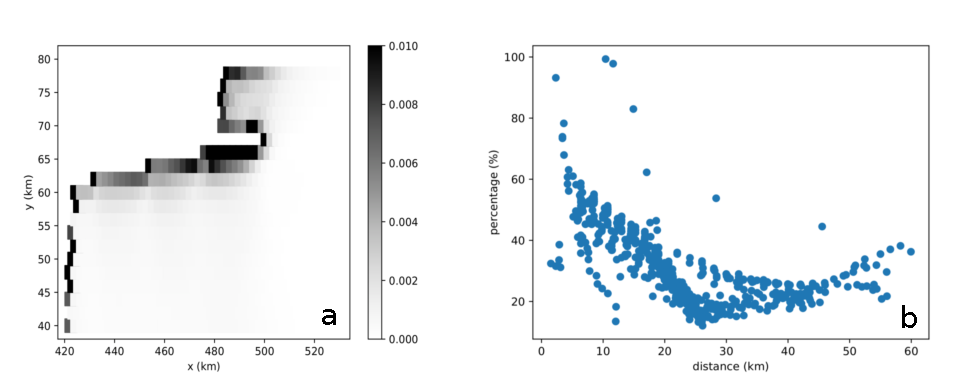
\includegraphics[width=1\linewidth]{figs/stndVarFluxP.pdf}
%\caption{(a) The distribution of the standard variance of the ice velocity changes on the grounding line of MISMIP+ for all perturbation experiments (note we only do the perturbation experiments for half space in $y$ of MISMIP+); (b) We find five cells on the grounding line that are the nearset to the perturbation spot. The x-axis is their mean distances to the perturbation box. The y-axis shows their combined flux contribution in the total integrated grounding line flux.}
%\label{stndVarFluxP}
%\end{figure}

%This can be further examined by looking at the relationship between GL flux response number ($N_r$) and the buttressing number ($N_b$) for the first principle stress ($\sigma_{p1}$) at different $dG$ and $dC$ (Fig \ref{diffdCdG}). $dG$ ($dC$) is the minimum distance between perturbation boxes and GL (calving front). When both $dG$ and $dC$ increase, perturbation boxes are farther away from GL and calving front, the velocity changes at GL become less dispersible and their relationship gets less ``noisy'' and tends to show linear trends. The possible explanaions can be found in the following ``Discussions'' section.

%\begin{figure}
%\centering
%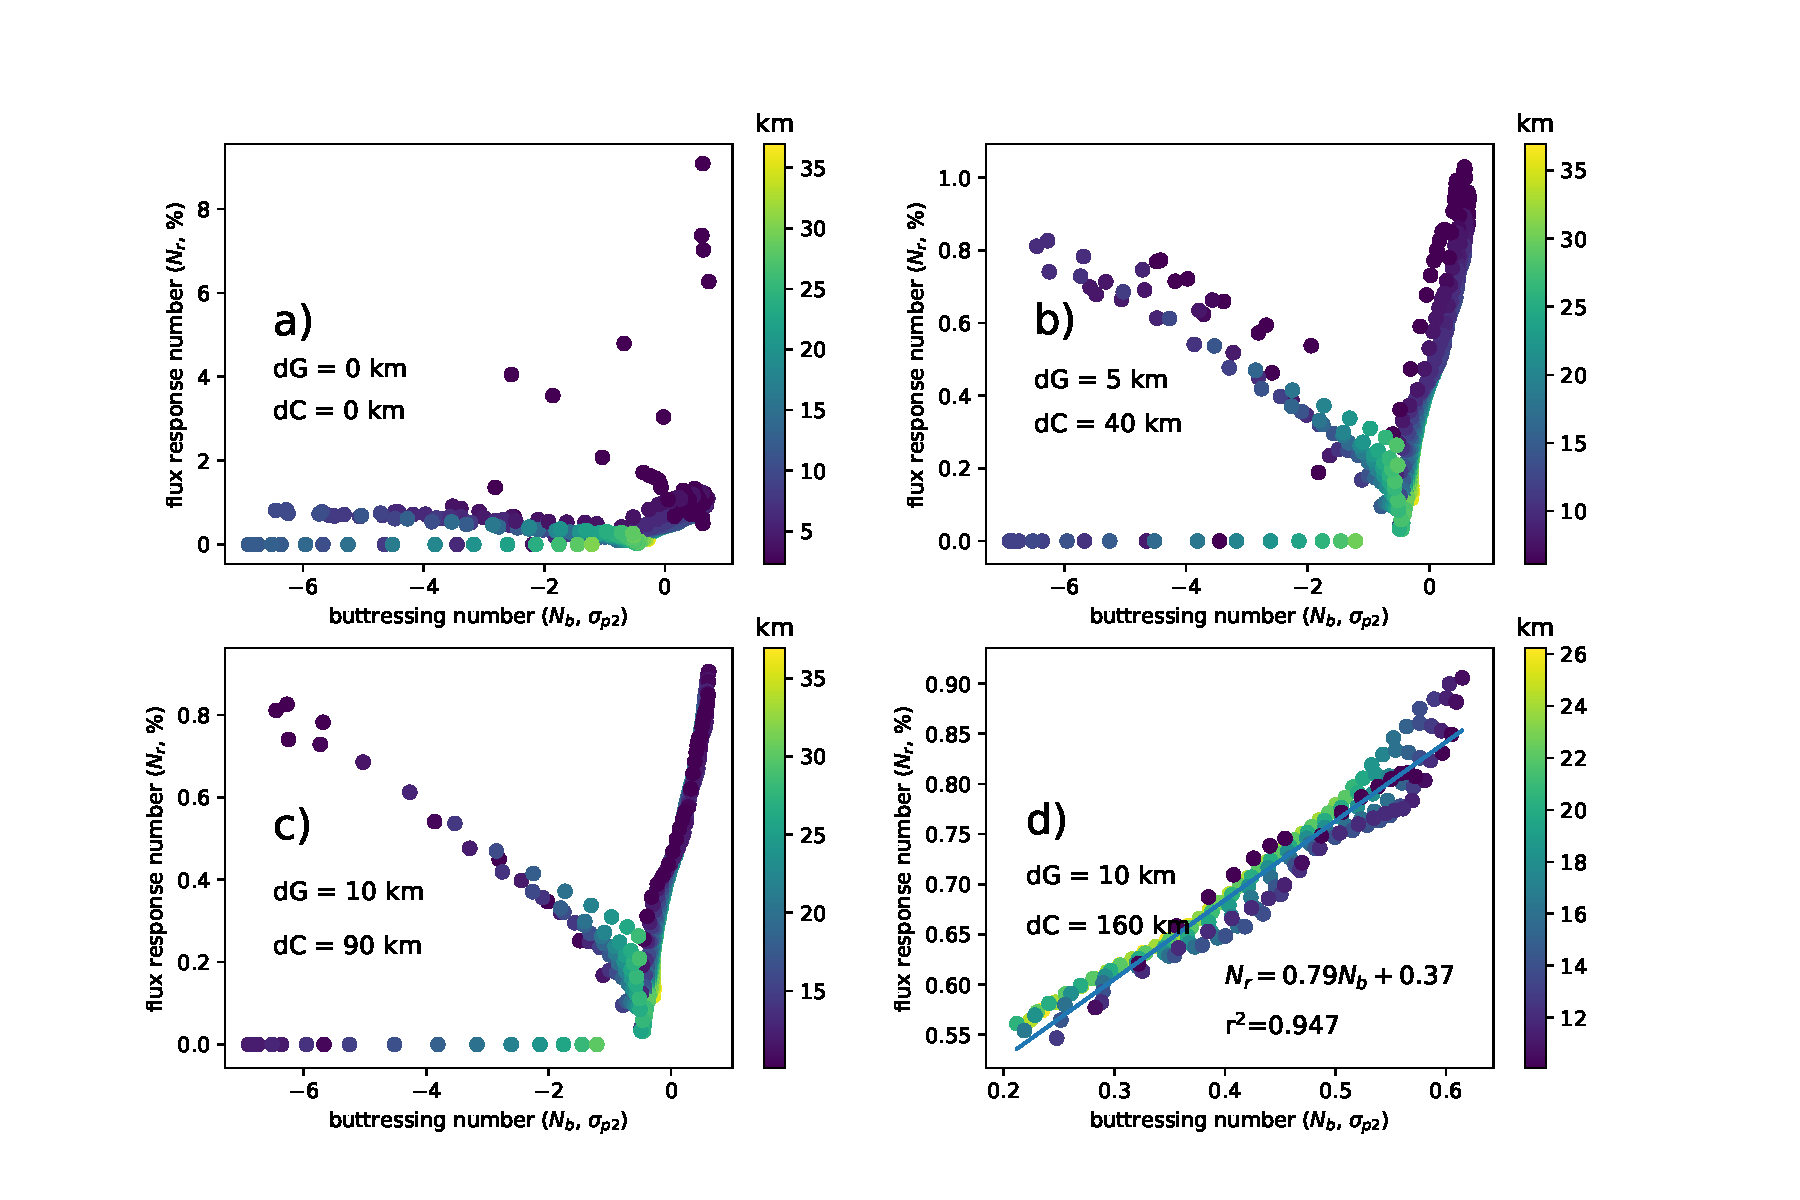
\includegraphics[width=1\linewidth]{figs/diffdCdG.pdf}
%\caption{The relationships between the groundling line flux response number ($N_r$) and the buttressing number ($N_b$) at the perturbation spots by different geometric filters of $dG$ and $dC$. Larger $dG$ and $dC$ give perturbation spots that are more centralized in the ice shelf. Smaller $dG$ and $dC$ mean the perturbation locations are either close to the grounding line or the calving front. The color bars show the values of $dG$ for each perturbation spot.}

%\label{diffdCdG}
%\end{figure}

%In fact, $\sigma_{p1}$ appears to be the best metric for predicting such linear relationship, comparing to the other 7 stress components (Fig \ref{diffStressComp}). The $N_b$ for $\sigma_f$, $\sigma_{af}$, $\sigma_x$ and $\sigma_y$ show some weak correlations with GL flux response number $N_b$. The shear stress and hoop stress, however, have no clear evidences of relating to $N_r$. Note that for all plots in Figure \ref{diffStressComp}, we have removed the ``noisy'' perturbation spots using $dG$ and $dC$. It is suprising that $\sigma_{p1}$ shows better performance than $\sigma_{p2}$ and $\sigma_s$, as $\sigma_{p2}$ gives the maximum buttressing number and predicts well the passive ice regions in \cite{furst2016} and the shear stress supply the main large resistence force for divergent ice flow regions (most of the MISMIP+ ice shelf) \citep{wearing2016}.

%\begin{figure}
%\centering
%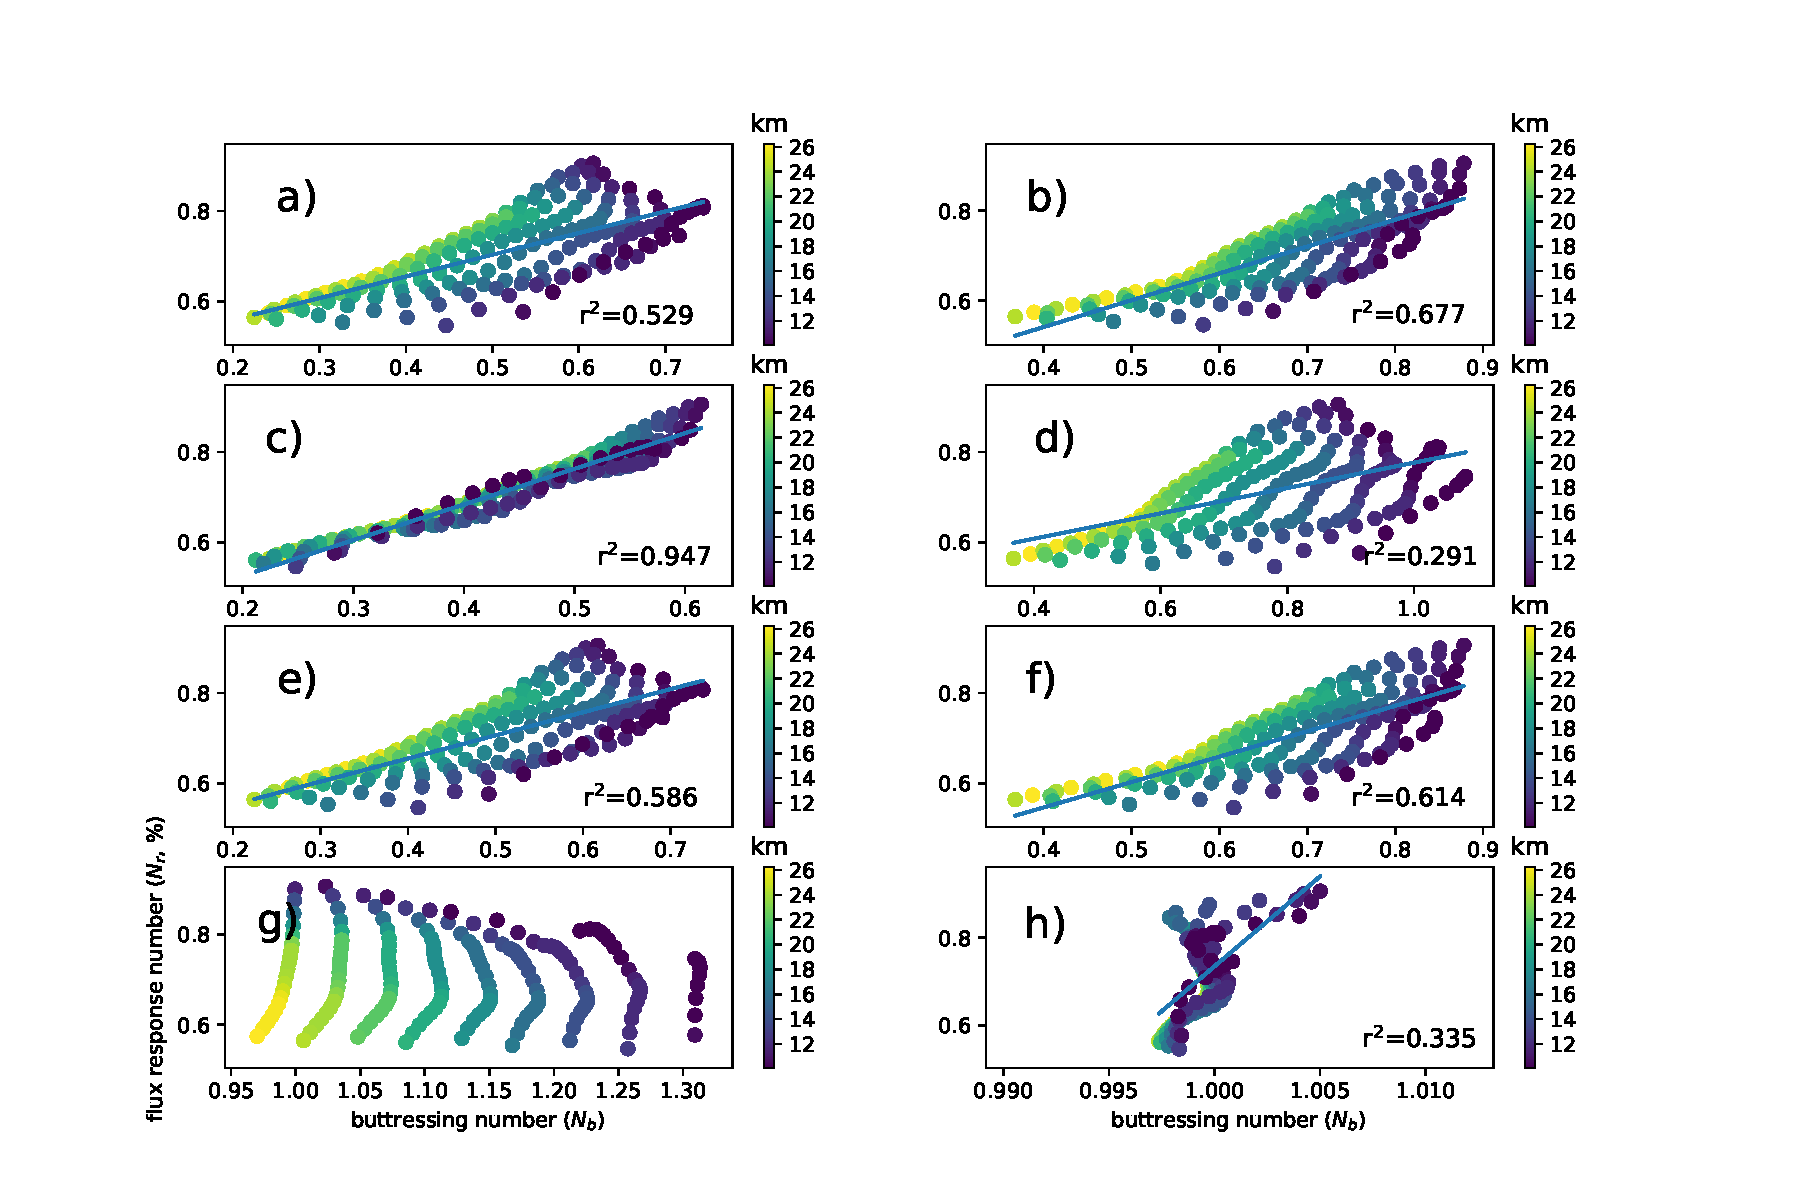
\includegraphics[width=1\linewidth]{figs/diffStressComp.pdf}
%\caption{The relationships between grounding line flux response number ($N_r$) and eight different stress components, $\sigma_f$ (a), $\sigma_{af}$ (b), $\sigma_{p1}$ (c), $\sigma_{p2}$ (d), $\sigma_{x}$ (e), $\sigma_{y}$ (f), $\sigma_{s}$ (g) and $\sigma_h$ (h). See Table \ref{stressDef} for the definition of each stress component in the MISMIP+ 2 km $\times$ 2 km box experiments. The color bars show the values of $dG$ for each perturbation spot.}
%\label{diffStressComp}
%\end{figure}

%The buttressing number for $\sigma_{p1}$ also performs well for the 10 km $\times$ 10 km square box perturbation experiments (Fig \ref{diffStressCompAvg}), for which we average the stresses across all cells in each square box. In fact, except the shear stress $\sigma_s$, all correlations are improved compared to the 2 km $\times$ 2 km perturbation experiments. In particular, the hoop stress shows some improved predictability as well. But again, $\sigma_{p2}$ is still not preferable than $\sigma_{p1}$.

%\begin{figure}
%\centering
%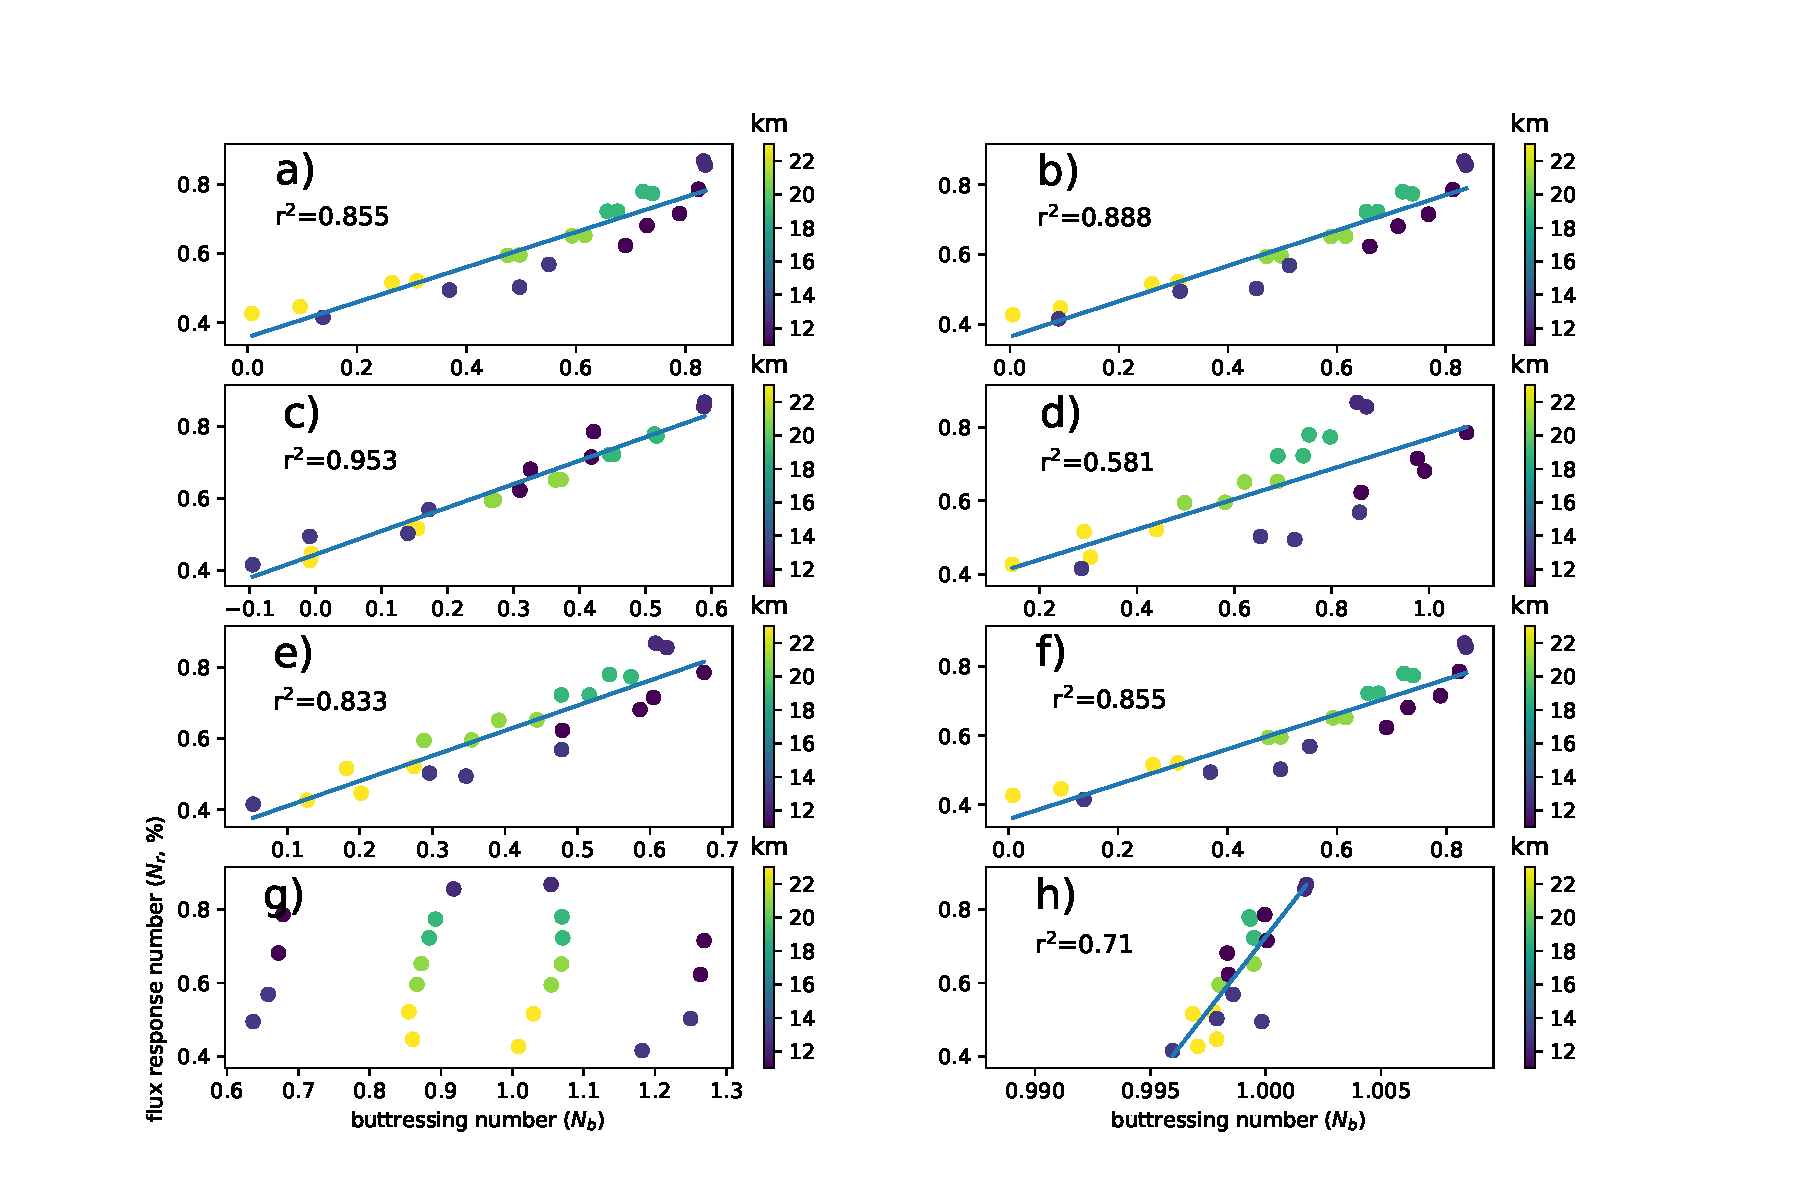
\includegraphics[width=1\linewidth]{figs/diffStressCompAvg.pdf}
%\caption{The relationships between grounding line flux response number ($N_r$) and eight different stress components, $\sigma_f$ (a), $\sigma_{af}$ (b), $\sigma_{p1}$ (c), $\sigma_{p2}$ (d), $\sigma_{x}$ (e), $\sigma_{y}$ (f), $\sigma_{s}$ (g) and $\sigma_h$ (h). See Table \ref{stressDef} for the definition of each stress component in the MISMIP+ 10 km $\times$ 10 km box experiments. The color bars show the values of $dG$ for each perturbation spot.}
%\label{diffStressCompAvg}
%\end{figure}


%\begin{figure}
%\centering
%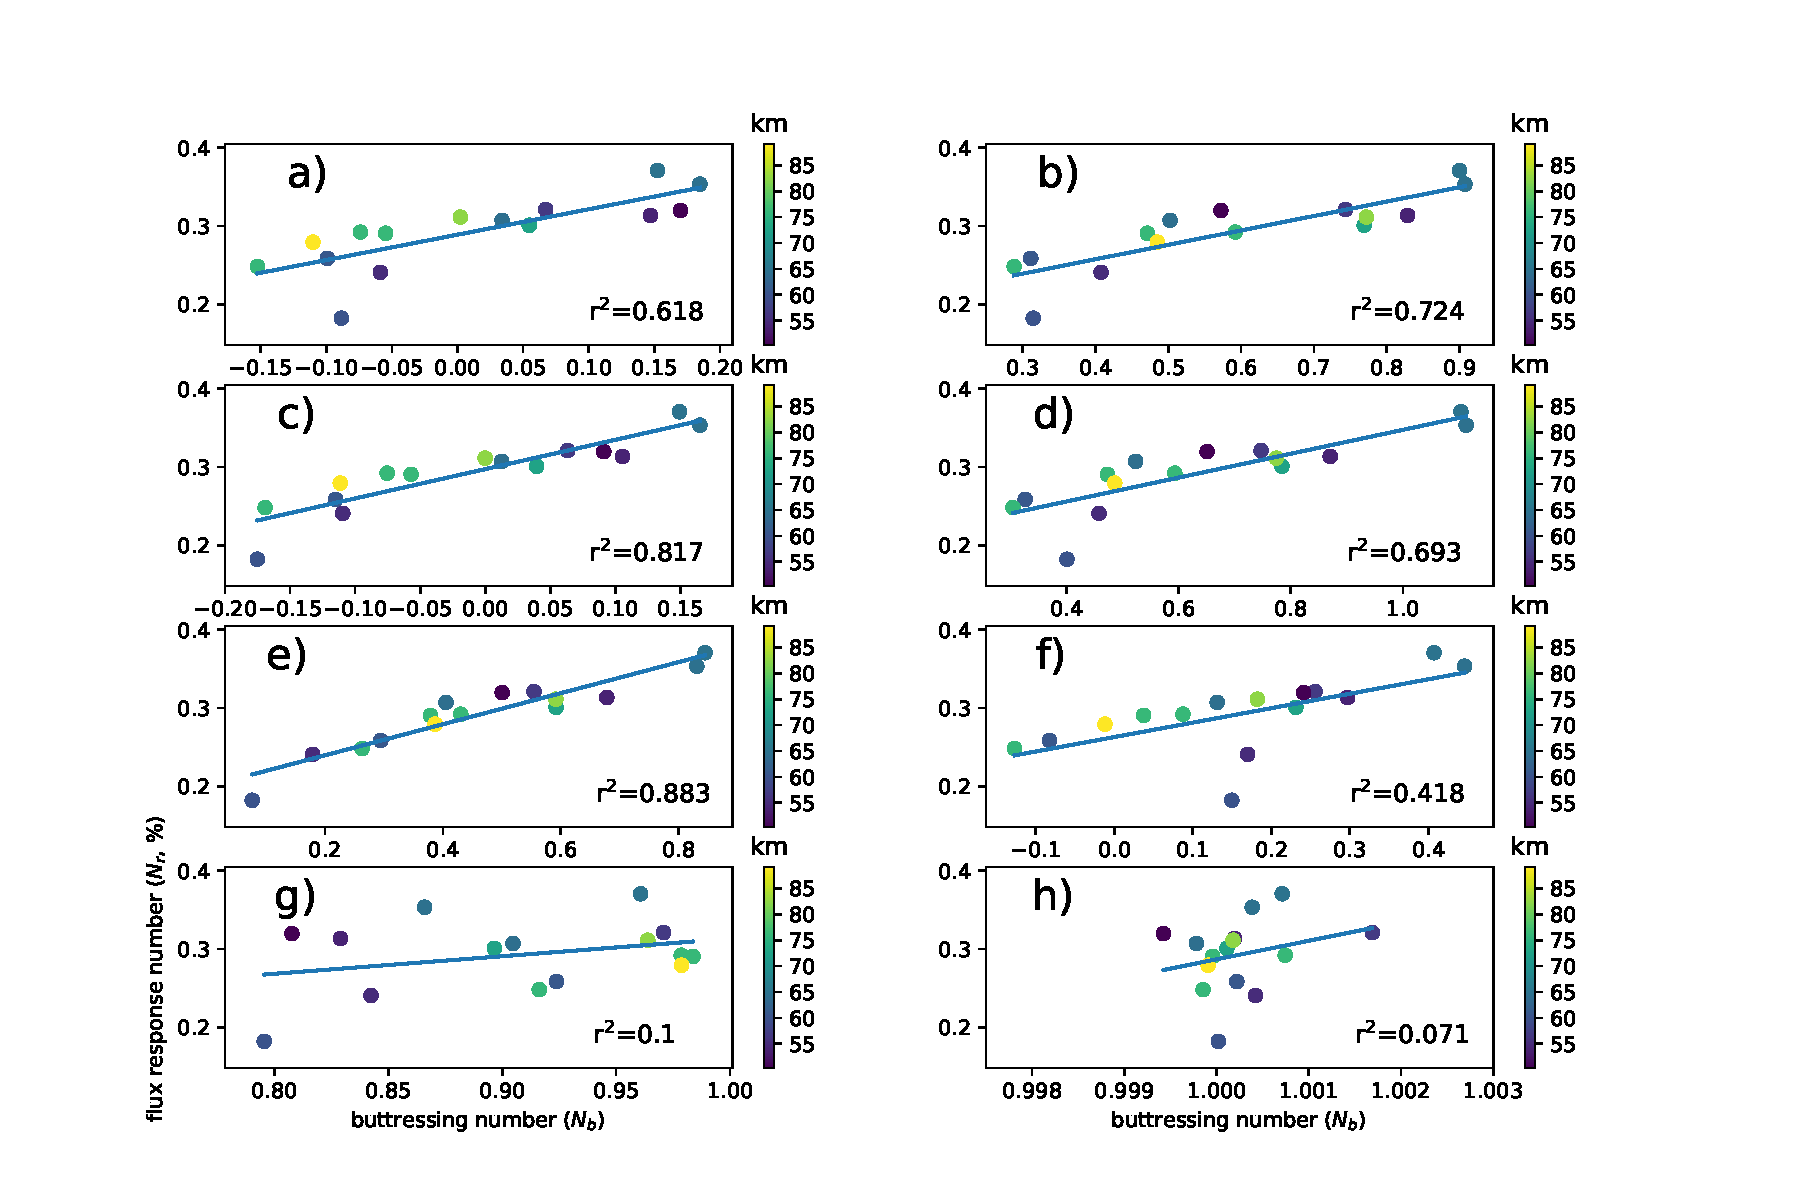
\includegraphics[width=1\linewidth]{figs/diffStressCompAvgL.pdf}
%\caption{The relationships between grounding line flux response number ($N_r$) and eight different stress components, $\sigma_f$ (a), $\sigma_{af}$ (b), $\sigma_{p1}$ (c), $\sigma_{p2}$ (d), $\sigma_{x}$ (e), $\sigma_{y}$ (f), $\sigma_{s}$ (g) and $\sigma_h$ (h). See Table \ref{stressDef} for the definition of each stress component in the Larsen C 20 km $\times$ 20 km box experiments. The color bars show the values of $dG$ for each perturbation spot.}
%\label{diffStressCompAvgL}
%\end{figure}

%Figure \ref{fig1} shows the relationships of integrated GL flux change and various buttressing numbers for different stresses for all perturbations over the MISMIP+ ice shelf. The inherent pattern is ambiguous. However, if we look closely to the distances of the perturbation points to GL, we can see the far scattered points are mostly near to the GL. Figure \ref{fig2} is an example of the impact of perturbation location on the velocity changes across the ice shelf and on GL. In addition to the complex velocity change patterns around the perturbation location, there are two clear patterns we can find: 1) the magnitude of vel. change decreased with distances away from the perturbation and 2) the vel. change pattern is different when the perturbation approaches to the GL. 

%The first one is easy to understand as the energy of perturbation decreases when it propagate away to far upstream and downstream. The second one can be explained by at least two mechanisms: 1) ice dynamics are more remarkably impacted by the grounded ice flow near the GL and 2) the propagation of perturbation can be more impacted by the spatial GL geometry. These two impacts can be confirmed if we remove the perturbation points both near the GL and in the open ice shelf area (little buttressing). See Figure \ref{fig3}, we only keep the perturbation points that are > 5 km away from the GL and also their x coordinates are < km 480 and some clear trends starts to appear. The buttressing number for shear and hoop stress seems to be not good metrics, but there are some relationships for $\sigma_{p1}$, $\sigma_{p2}$, $\sigma_f$, $\sigma_{af}$, $\sigma_x$ and $\sigma_y$, especially for $\sigma_{p1}$. 

%This can be further verified if we apply the perturbation to a spatial box (20km by 20 km) and calculate the average stress field in each perturbation box, by which we can smooth out and decrease the impacts of distances on the GL flux responses (Fig \ref{fig4}). the shear stress buttressing number is still a bad metric, but the averaged hoop stress turns out to become much better than the 2 km perturbation cell case. Other stresses along different directions also present better behaviors for GL flux responses.

%Based on the above MISMIP+ results, we apply the same approaches to Larsen C ice shelf. See Figure \ref{fig5}, though Larsen C has a more complex geometry compared to MISMIP+, it still show good linear relationship between the $\sigma_{p1}$ buttressing number and GL flux response. Different than the MISMIP+ runs, we remove the perturbation spots that are < 10km to the GL and calving front.



%\section{Discussions}
%
%Based on the above discussion we hypothesize that the two main factors controlling how a local perturbation in ice shelf thickness leads to changes in ice flux across the GL are 1) the distance between a perturbation location and the GL and 2) the first principle stress at the perturbation location. Figure \ref{distPerturbComp} shows an example of the impact of the perturbation location on the velocity changes across the ice shelf and GL. Despite the complex patterns of velocity change around the perturbation spot, we can see two clear features: 1) the magnitude of velocity change decreases with distances away from the perturbation spot and 2) the velocity change pattern becomes different and more disordering when the perturbation  approaches to GL. 
%
%
%The first feature is easy to understand because the energy of perturbation decays as it propagate away to far upstream and downstream. However, the perturbation propagation is not simply dependent on distance, but replies on the ice flow field. A complete perturbation propagation theory is necessary to describe/explain these small velocity changes across the ice shelf, however, it is beyond the scope of this study. The second one can probably be explained by two ice-flow mechanisms: 1) ice shelf dynamics are remarkably impacted by the grounded ice flow near the GL since it's a coupled system for grounded ice sheet and floating ice shelf and in MALI they is resolved as an integrated system as well; 2) the propagation of perturbation can be impacted by the spatial GL geometry. For example, the perturbation in Figure \ref{distPerturbComp}a can not directly impact the ice on the other side of the grounded peninsula in the same way as for it's neighboring cells.
%
%In addition, the impacts of distance can also be verified from the box averaging experiments (Figure \ref{diffStressCompAvg} and \ref{diffStressCompAvgL}). By smoothing out the stresses in the perturbation box, different distances to GL for each cells and their impacts in the perturbation box are also averaged, resulting in better linear $N_b$-$N_r$ relationships. This possibly indicates that those linear $N_b$-$N_r$ relationships can apply for realistic ice shelves, as in reality the basal melting always occurs in wide spatial regions.
%
%%These two impacts can be confirmed if we remove the perturbation points both near the GL and in the open ice shelf area (little buttressing). See Figure \ref{fig3}, we only keep the perturbation points that are > 5 km away from the GL and also their x coordinates are < km 480 and some clear trends starts to appear. The buttressing number for shear and hoop stress seems to be not good metrics, but there are some relationships for $\sigma_{p1}$, $\sigma_{p2}$, $\sigma_f$, $\sigma_{af}$, $\sigma_x$ and $\sigma_y$, especially for $\sigma_{p1}$. 
%
%It is still not very clear why the integrated GL flux change is strongly correlated to the first principle stress at the perturbation location than other stress components (especially the second principle stress). We can find some clues by looking at the difference of $\sigma_{p1}$, $\sigma_{p2}$, $\sigma_f$ and $\sigma_s$ along GL before and after applying the perturbation (Fig \ref{stressDiff}). Clearly, the distribution of the difference of $\sigma_{p1}$ across ice shelf is less disordering than that of $\sigma_{p2}$, $\sigma_{f}$ and $\sigma_{s}$. This indicates that the propagation of the perturbation for different stress components can be greatly varied in patial, which is probably the main reason of those different $N_b$-$N_r$ relationships for different stress components. A further evidence of this explanation can be found in Figure \ref{stressDiff_velDiff}, where we show the changes of veocity and stress components on GL. Clearly, the change of ice speeds at GL is more relevant to of $\sigma_{p1}$ and $\sigma_{f}$, compared to $\sigma_{p2}$ and $\sigma_{s}$. This possibly indicate that the changes of ice velocity under small basal perturbations may be more likely controlled by the changes of the stress components that are more aligned with ice flow directions.
%
%
%Therefore, we can find similar patterns for shear stress $\sigma_s$. The ice flow for most parts of MISMIP+ and Larsen C ice shelf are divergent, which in practical don't supply any buttressing to resist along flow. Since the hoop stress is quite small (Fig \ref{diffStressCompAvg}h and Fig \ref{diffStressCompAvgL}h), the main source of buttressing arises from the shear flow of ice shelf (assume the buttressing is proportional to the magnitude of $\sigma_{obj}$). This can be confirmed in \citep{furst2016} where we can clearly see that some non-passive (with buttressing) ice shelf are purely extensive regime. Similar to the case of $\sigma_{p2}$, the complex spatial propagation of the perturbed stress change from the perturbation spot to GL is a possible cause.
%
%
%
%
%%From Figure \ref{fig2} we can see the ice vel. change over ice shelf and GL depends on the relative location to GL position. When p is near the center of the ice shelf, the ice flux change is more predictable than p close to the GL. The magnitude of vel. change decrease with distance, and the vel. upstream (downstream) tends to show an increase (decrease). For the ice shelf (GL) upstream to the perturbation, a decrease of ice thickness indicates a decrease of buttressing, however, for ice shelf downstream to the perturbation, it means a decrease of driving stress. This pattern become ambiguous when the perturbation is close to GL as it's dynamics is more affected by the grounded ice sheet. 
%
%
%Though there is no clear linear $N_b$-$N_r$ relationships near GL, the integrated GL flux mainly depends on the GL flux of cells that are close to the perturbation spot. From Figure \ref{stndVarFluxP}b, we can see that for perturbations near GL, their impacts are mainly local and thus can only affect their neighboring ice streams, which can possibly enhance the spatial heterogeneity of marine ice sheet responses under ocean warming forcings.  


\section{Conclusions}

From this study we find that the sensitivity of grounding line (GL) flux to melt perturbations beneath ice shelves appears to be linearly related to the buttressing number for certain stress field of the ice flow regime when the perturbations are located near the center of ice shelves. We can divide an ice shelf into three different geometric regions: 1) near GL where the shear margins dominate; 2) near the calving fronts where ice can be considered as ``passive'' and 3) the central regions of ice shelf. Though it is ambiguous to indentify the boundaries of those three sub-regions, we find that both the shear margins and passive ice regions show very weak linear connections to GL flux changes. The shear margins are strongly impacted by the upstream grounded stream flows and the passive ice shelf basically has negligible contribution to GL dynamics. 

The buttressing of ice shelf resists ice flows from upstream. The maximum buttressing number (calculated from the second principle stress $\sigma_{p2}$) is a commonly used metric to quantify the buttressing effects of ice shelf, doesn't show clear correlations to the changes of GL flux. Among many possible factors we find that the distance away from perturbation locations may be a critical control for perturbation propagation across ice shelves, which is important for understanding the relationships between the stress field of the ice shelf and the GL flux changes. The GL ice speed changes may be more correlated to the changes of the first principle stress ($\sigma_{p1}$) and normal stress along flow ($\sigma_{f}$) than other stress components, for example, the second principle stress ($\sigma_{p2}$) and the shear stress ($\sigma_s$), indicating that the stress component ($\sigma_{p2}$) that contribute significantly to buttressing is not necessarily related to the progapation of buttressing. 

The linear $N_b$-$N_r$ relationships presented in this study are based on small (1 m) thickness perturbations. However, it's still unclear if they can stand for large melts at the bottom of ice shelves ({\bf{Perhaps we also need to do large perturbation experiments?}}). Despite the progress we have made in this study, we suggest to apply a fully-developed perturbation propagation model for further understanding the physics of GL flux changes under ocean forcings. 

\section{Acknowledgement}
\bibliographystyle{igs}
\bibliography{refs}

\section{Appendix}

%\renewcommand\thefigure{\thesection.\arabic{figure}}  
\renewcommand{\thefigure}{A\arabic{figure}}
\setcounter{figure}{0}

%\begin{figure}
%	\centering
%	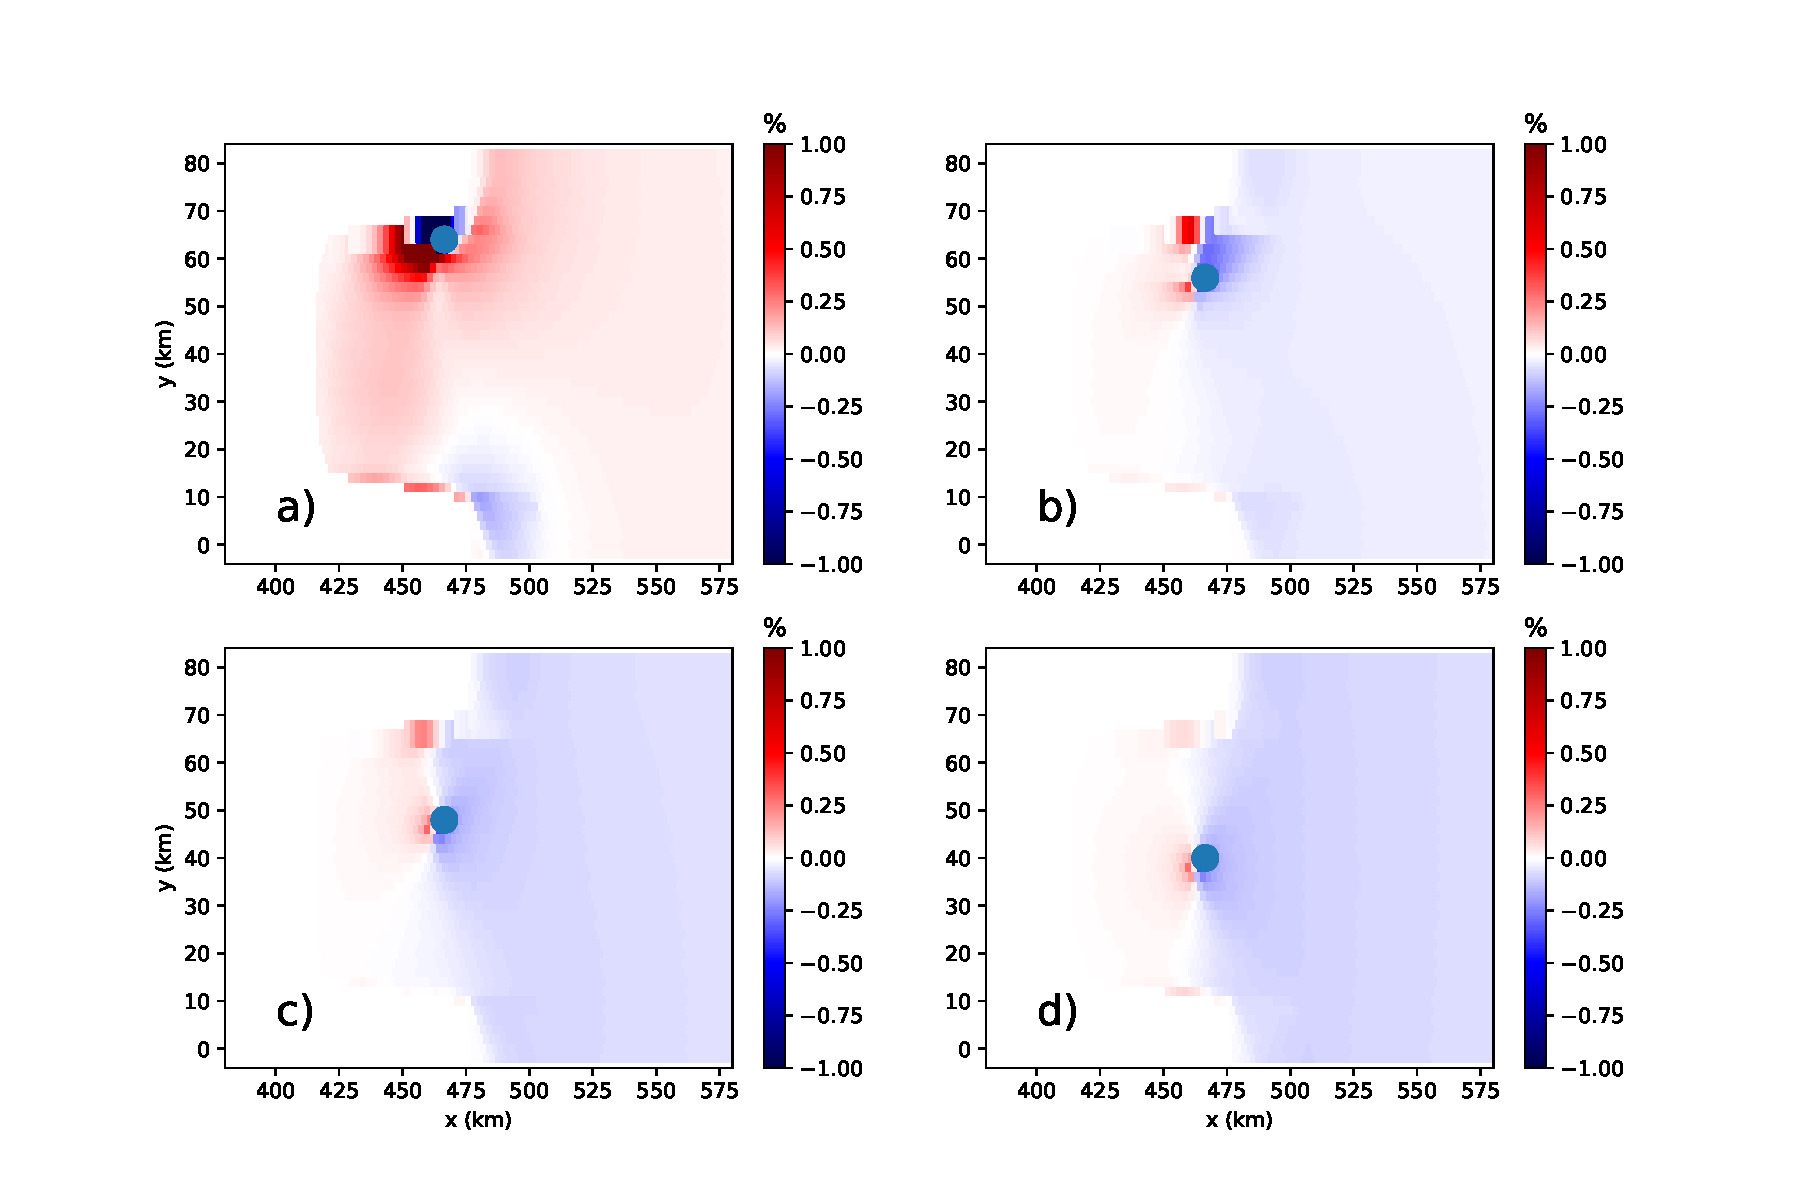
\includegraphics[width=1\linewidth]{figs/distPerturbComp.pdf}
%	\caption{An example of ice speed changes (\%) across the MISMIP+ ice shelf and grounding line after apply the perturbations at different locations (blue circles).}
%	\label{distPerturbComp}
%\end{figure}
%
%\begin{figure}
%	\centering
%	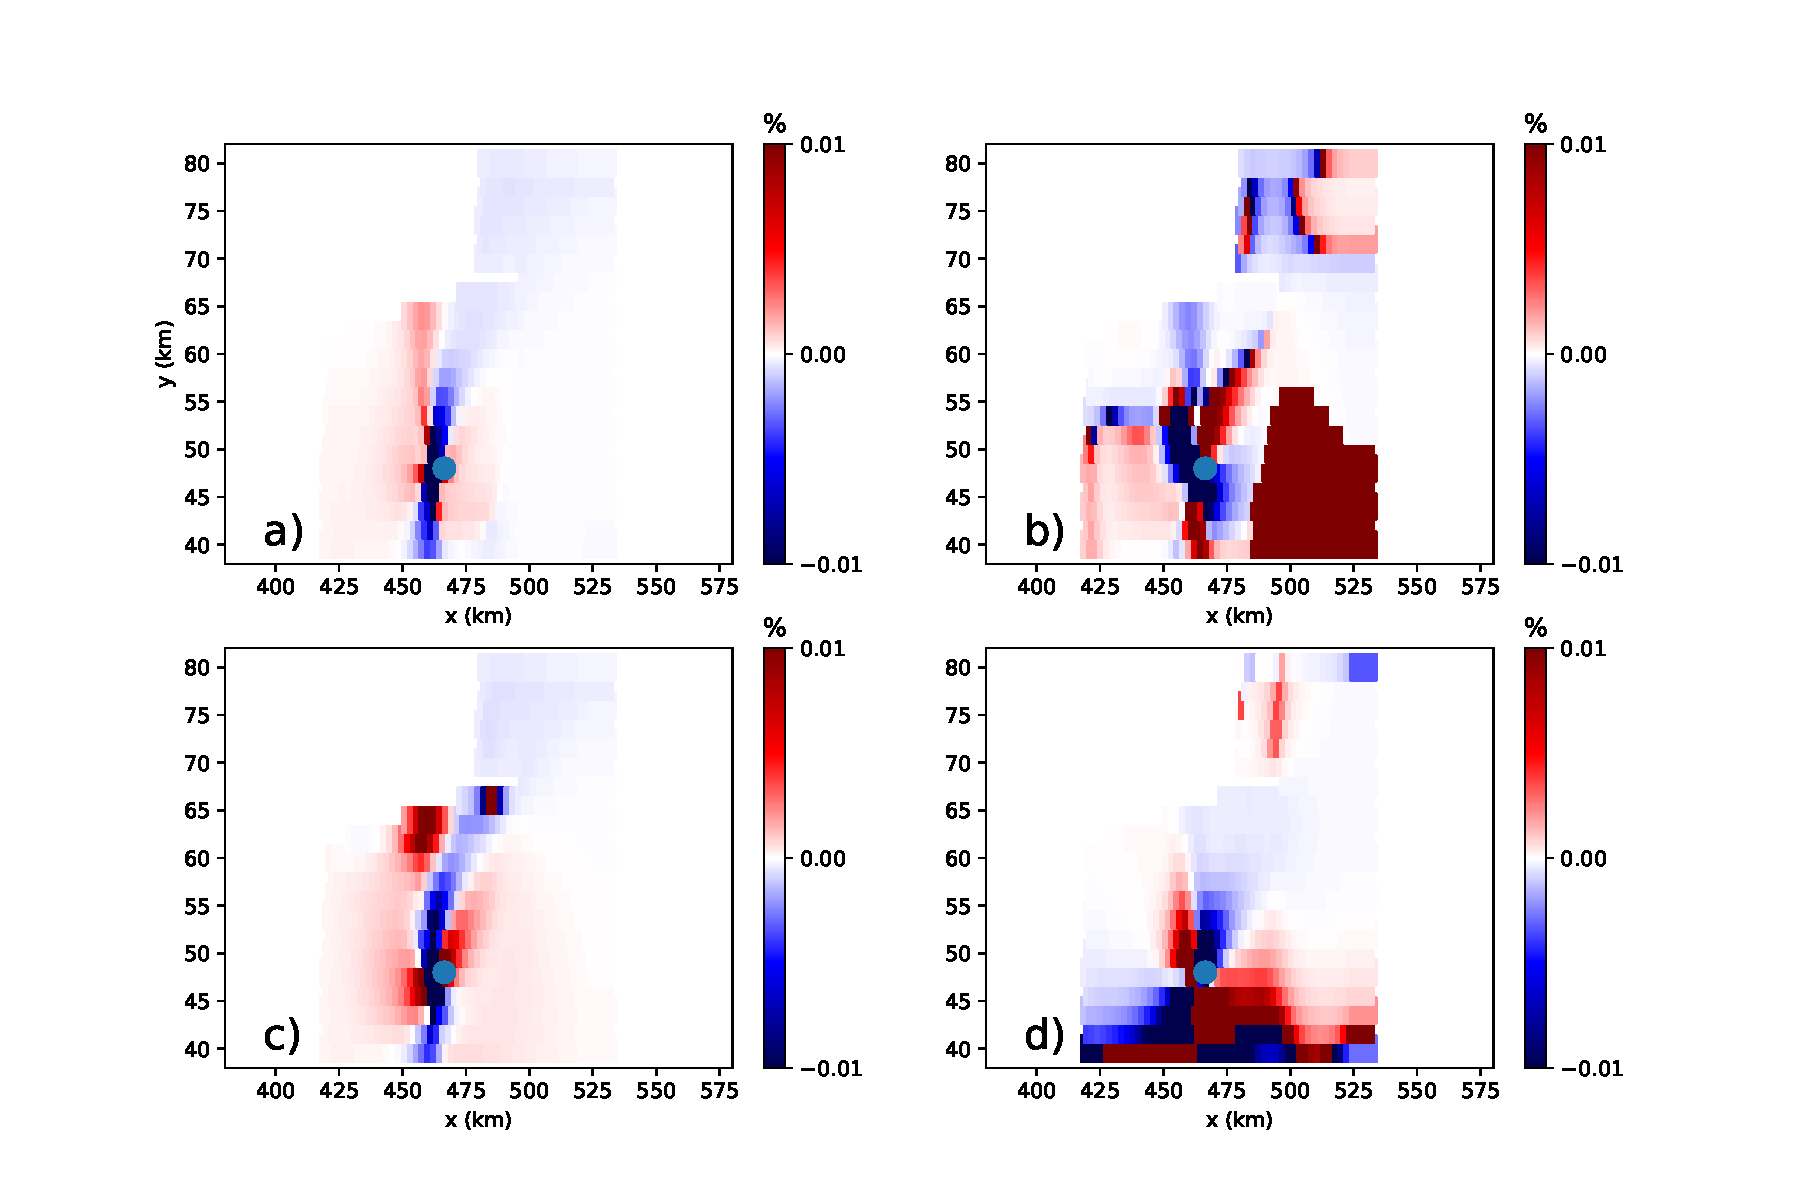
\includegraphics[width=1\linewidth]{figs/stressDiff.pdf}
%	\caption{An example of stress component changes (\%) across the MISMIP+ ice shelf and grounding line after apply the perturbations at different locations (blue circles). (a) Changes of $\sigma_{p1}$; (b) Changes of $\sigma_{p2}$; (c) Changes of $\sigma_{f}$; (d) Changes of $\sigma_{s}$;.}
%	\label{stressDiff}
%\end{figure}
%
%\begin{figure}
%	\centering
%	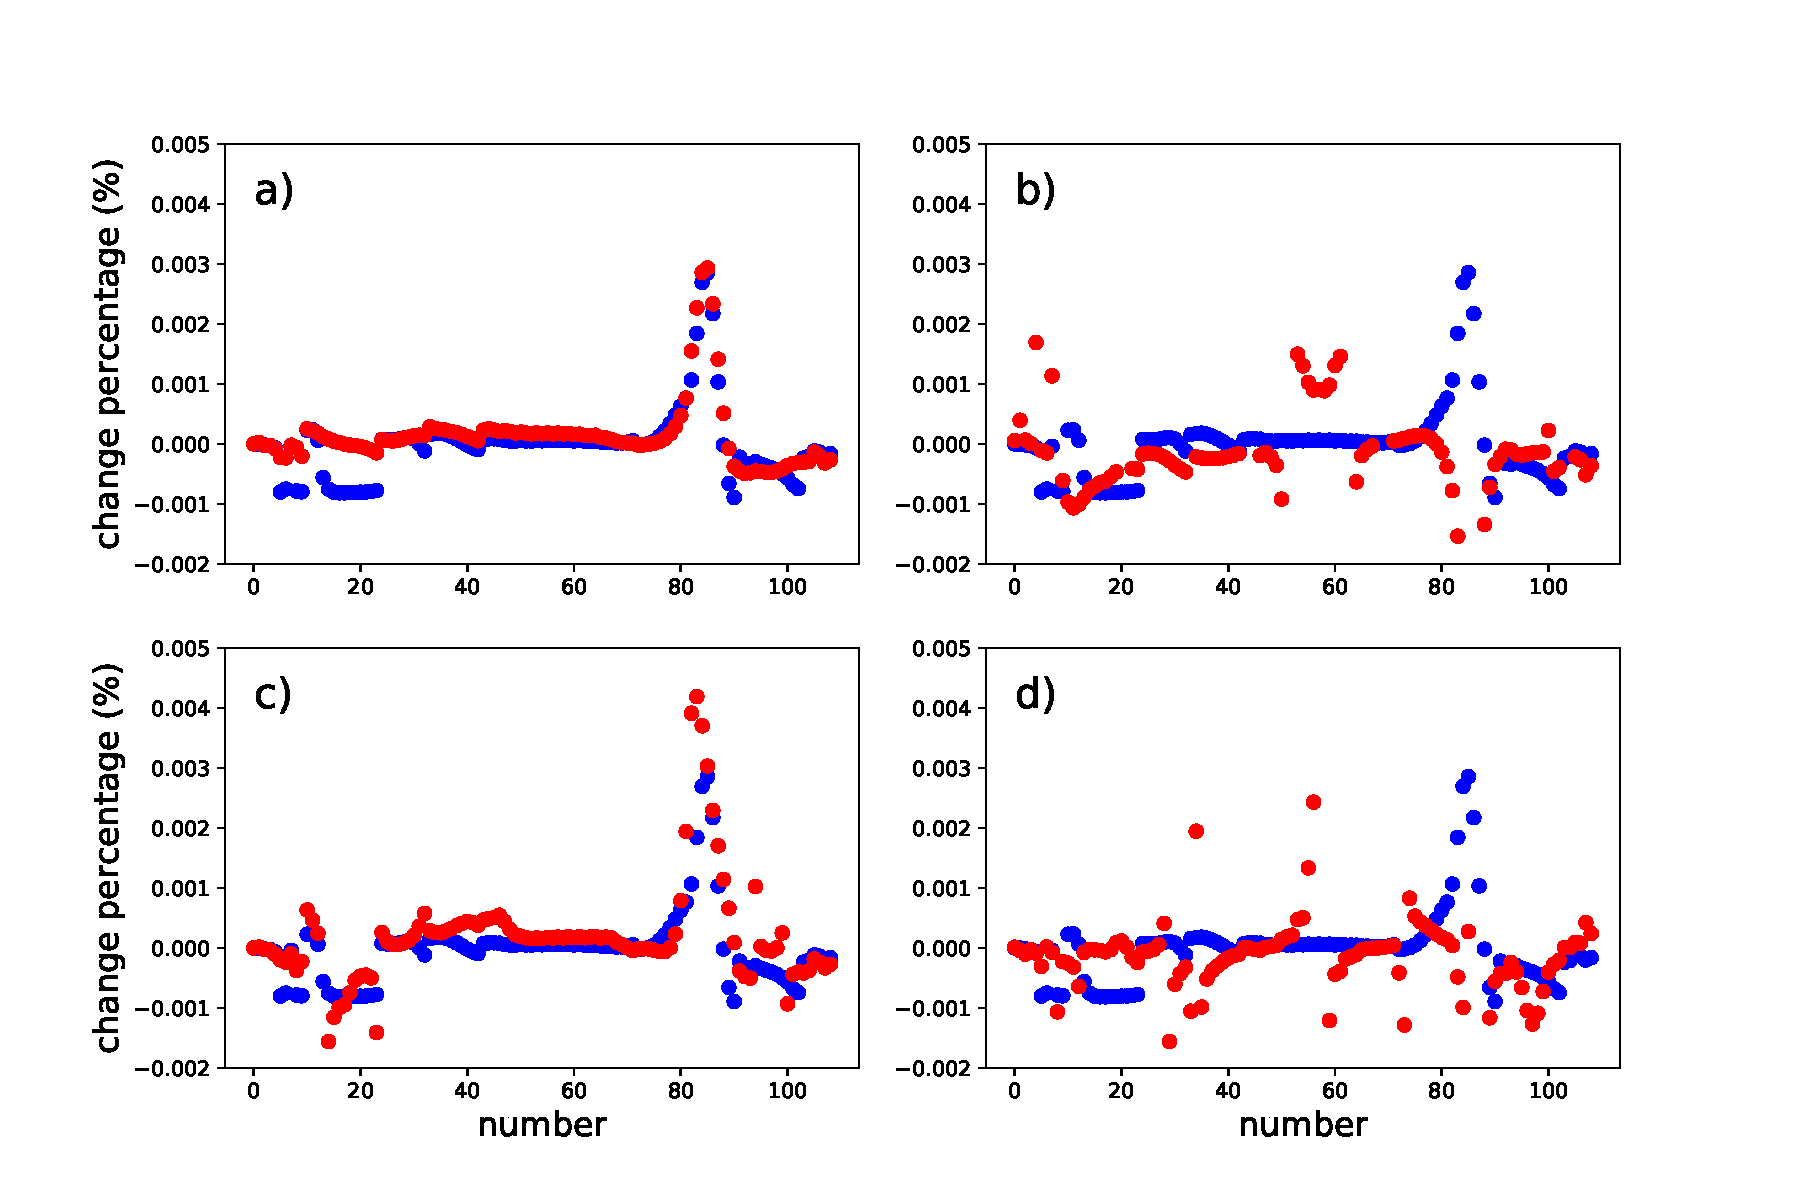
\includegraphics[width=1\linewidth]{figs/diffStress_diffVel.pdf}
%	\caption{The change percentage of ice speed (blue dots) and stress components (red dots; a--d represents $\sigma_{p1}$, $\sigma_{p2}$, $\sigma_{f}$ and $\sigma_{s}$, respectively) for all cells at the grounding line corresponding to Figure \ref{stressDiff}.}
%	\label{stressDiff_velDiff}
%\end{figure}

\end{document}
